\documentclass{memoir}
\usepackage{notestemplate}
\usetikzlibrary{arrows,chains,matrix,positioning,scopes}

\makeatletter
\tikzset{join/.code=\tikzset{after node path={%
\ifx\tikzchainprevious\pgfutil@empty\else(\tikzchainprevious)%
edge[every join]#1(\tikzchaincurrent)\fi}}}
\makeatother

\tikzset{>=stealth',every on chain/.append style={join},
         every join/.style={->}}


\logo{~/LibreMath/Auxiliary Resources/resources/png/logo.png}
\institute{Rice University}
%\faculty{Faculty of Whatever Sciences}
\department{Department of Mathematics}
\title{Introduction to Module Theory}
%\subtitle{Based on MATH xxx}
\author{\textit{Author}\\Gabriel \textsc{Gress}}
%\supervisor{Linus \textsc{Torvalds}}
%\context{Well, I was bored...}
\date{\today}

%\makeindex

\begin{document}

\maketitle

% Notes taken on 
\setcounter{chapter}{-1}
\chapter{Preamble}
\label{cha:preamble}

\documentclass{memoir}
\usepackage{notestemplate}

%\logo{./resources/pdf/logo.pdf}
%\institute{Rice University}
%\faculty{Faculty of Whatever Sciences}
%\department{Department of Mathematics}
%\title{Class Notes}
%\subtitle{Based on MATH xxx}
%\author{\textit{Author}\\Gabriel \textsc{Gress}}
%\supervisor{Linus \textsc{Torvalds}}
%\context{Well, I was bored...}
%\date{\today}

\begin{document}

% \maketitle

% Notes take on 01/25/21

\chapter{Introduction}
\label{cha:introduction}

These notes covers modules, unital and commutative rings, and fields.\\

The lecture notes are based off two main sources. The overall outline and the major statements of theorems and definitions are based off lecture notes from Dr.\@ Chelsea Walton during the Spring 2021 teaching of Rice's course MATH 357 -- \textit{Abstract Algebra II}. These notes are supplemented by exercises from Dummitt and Foote's \textit{Abstract Algebra}, and some of the basic ring material is based on Goodman's \textit{Algebra: Abstract and Concrete}. Finally, the applications of Galois theory are based on a section from Hungerford's \textit{Algebra}.

\end{document}


\chapter{Introduction to Modules}
\label{cha:introduction_to_modules}

\documentclass{memoir}
\usepackage{notestemplate}
%\logo{./resources/pdf/logo.pdf}
%\institute{Rice University}
%\faculty{Faculty of Whatever Sciences}
%\department{Department of Mathematics}
%\title{Class Notes}
%\subtitle{Based on MATH xxx}
%\author{\textit{Author}\\Gabriel \textsc{Gress}}
%\supervisor{Linus \textsc{Torvalds}}
%\context{Well, I was bored...}
%\date{\today}

\begin{document}

% \maketitle

% Notes taken on 02/05/21

\section{Modules}
\label{sec:modules}

An \(R\)-module \(M\) is an abelian group that comes equipped with a binary operation \(\cdot \) that maps from \(R\times M\) to \(M\) that is compatible with operations of both \(M\) and \(R\). It is the natural generalization of vector spaces to rings, but with the key difference that we may not have multiplicative inverses for elements in our \(R\)-module.

\begin{defn}[Left \(R\)-module]
Let \(R\) be a ring. A \textbf{left \(R\)-module} is a pair \(\prescript{}{R}{M} := (M,\cdot :R\times M\to M)\) where \(M\) is an abelian group, and \(\cdot \) is a binary operation so that
	\begin{align*}
		\forall r,s \in R, \; m,n \in M:\\
		r\cdot (m+n) = (r\cdot m) + (r\cdot n)\\
		(r+s)\cdot m = (r\cdot m) + (s\cdot m)\\
		(rs)\cdot m = r\cdot(s\cdot m)
	\end{align*}
	If \(R\) is unital, then we also require
	\begin{align*}
		1_R \cdot  m = m.
	\end{align*}
	The map is called the (left) \textbf{\(R\)-action map}.
\end{defn}

\begin{exmp}[Free Module of Rank \(n\)]
	\begin{enumerate}
		\item If \(R\) is a field \(F\), then the \(R\)-module is an \(F\)-vector space.
		\item Take \(M = R^{n} := \left\{(t_1,\ldots,t_n) \mid t_i \in R \right\}\). Let the \(R\)-action map of \(\prescript{}{R}M\) be defined by
			\begin{align*}
				R\times M \to M\\
				(r,(t_1,\ldots,t_n)) \mapsto (rt_1,\ldots,rt_n).
			\end{align*}
			One can check that this satisfies the necessary properties of a left \(R\)-action on \(M = R^{n}\). This left \(R\)-module \(\prescript{}{R}R^{n}\) (which we will simply denote here on out by \(R^{n}\)) is called the \textbf{free left \(R\)-module of rank \(n\)}.
	\end{enumerate}
\end{exmp}

\begin{exmp}[\(\Z\)-Modules]
An abelian group \(M\) can be made into a module \(\prescript{}{\Z}M\) over the integers in exactly one way. Consider the \(\Z\)-action map defined by
\begin{align*}
	\Z\times M \to M\\
	(n,m) \mapsto  m + \ldots_{n} + m
\end{align*}
One can check that this indeed is a \(\Z\)-module over \(M\). 
\end{exmp}

\begin{hw}
	Prove that the \(\Z\)-action given above is the unique \(\Z\)-action for any \(\Z\)-module. Furthermore, show that \(\prescript{}{\Z}M\) is isomorphic to an abelian group.
\end{hw}

\begin{exmp}[\(F{[}x{]}\) Modules]
	Let \(R = F[x]\) be a polynomial ring over a field \(F\), and let \(V\) be a vector space over \(F\) with a linear operator \(T \in \mathcal{L}(V)\). We can construct an \(F[x]\)-module on \(V\) via \(T\) (denoted \(\prescript{}{F[x]}V)\)). To see this, let \(p(x) \in F[x]\) be a polynomial given by
	\begin{align*}
		p(x) = a_nx^{n}+ a_{n-1}x^{n-1} + \ldots + a_1 x + a_0.
	\end{align*}
	For each \(v \in V\), we define the action of \(p(x)\) on \(v\) by
	\begin{align*}
		p(x)\cdot v &= (a_n T^{n} + a_{n-1}T^{n-1} + \ldots + a_1 T + a_0) (v)\\
		       &= a_n T^{n}(v) + a_{n-1}T^{n-1}(v) + \ldots + a_1 T(v) + a_0v
	\end{align*}
	Informally, we are defining an action of \(x\) on \(V\) by \(T\), and then extending it onto \(F[x]\) in a natural way.\\

	Recall that \(F\leq F[x]\) (as constant polynomials), and hence the action of \(F\) is exactly the same as constant polynomials, which correspond to the standard action of \(F\) on \(V\). In other words, this action is an extension of the action of \(F\) onto a larger ring \(F[x]\).\\

	Because this action is dependent on the choice of  \(T\), this gives us many different \(F[x]\)-module structures on the same vector space \(V\). One can check that \(T=0\) also yields us the standard action of \(F\) on \(V\).\\

	What is interesting to note is that the action of \(F[x]\) via \(T\) encapsules \textit{all} possible \(F[x]\)-modules-- this holds because the action of \(x \in F[x]\) on \(V\) is a linear transformation from \(V\) to \(V\), and hence must correspond to some \(T\) which all actions \(p(x)\) must adhere to.\\

	One might ask what \(F[x]\)-submodules look like. We can see immediately that an \(F[x]\)-submodule \(\prescript{}{F[x]}W \leq \prescript{}{F[x]}V\) must also be an \(F\)-submodule, and hence \(W<V\) as a vector subspace. Furthermore, in order for it to be well-defined, \(W\) must be \textbf{\(T\)-invariant}, that is, \(T(W) \subset  W\). In fact this too is a bijection, so that all \(F[x]\)-submodules of \(V\) correspond to \(T\)-invariant subspaces of \(V\).
\end{exmp}
This example shows that the ideal structure of \(F[x]\) greatly restricts the module structure on \(V\) (and in fact can be used to derive its Jordan canonical form). In fact, the reasonings above can be applied to any PID \(R\), and in the special case \(R = \Z\) we can obtain the fundamental theorem of finitely generated abelian groups. In general, it is always interesting to see how the structure of a ring \(R\) will affect its modules.

\end{document}

\documentclass{memoir}
\usepackage{notestemplate}

%\logo{./resources/pdf/logo.pdf}
%\institute{Rice University}
%\faculty{Faculty of Whatever Sciences}
%\department{Department of Mathematics}
%\title{Class Notes}
%\subtitle{Based on MATH xxx}
%\author{\textit{Author}\\Gabriel \textsc{Gress}}
%\supervisor{Linus \textsc{Torvalds}}
%\context{Well, I was bored...}
%\date{\today}

\begin{document}

% \maketitle

% Notes taken on 02/05/21

\section{Substructures of Modules}
\label{sec:substructures_of_modules}

\begin{defn}[Submodule]
	Let \(R\) be a ring, let \(\prescript{}{R}M\) be a left \(R\)-module, and let \(N\leq M\) be a subgroup of \(M\). A \textbf{\(R\)-submodule of \(\prescript{}{R}M\)} is the \(R\)-module \(\prescript{}{R}N\) with the same \(R\)-action from \(\prescript{}{R}M\).\\

	In other words, it is a subgroup with closure under the \(R\)-action.
\end{defn}

\begin{prop}[Submodule Criterion]
	Take a ring \(R\) with \(1_R\), and left \(R\)-module \(M\). A subset \(N\) of \(M\) can be made into a \(R\)-submodule of \(M\) if and only if
	\begin{itemize}
		\item \(N \neq \emptyset\) and
		\item \(n+rn' \in N\) for all \(r \in R\), \(n,n' \in N\).
	\end{itemize}
\end{prop}

\begin{prop}
	Let \(M\) be an \(R\)-module, and let \(\prescript{}{R}N_{i}\) with \(i \in I\) be \(R\)-submodules of \(M\). Then
	\begin{enumerate}
		\item \(\bigcap_{i \in  I} \prescript{}{R}N_i\) is an \(R\)-submodule of \(M\) 
		\item \(\bigcup_{i \in  I} \prescript{}{R}N_i\) is not necessarily an \(R\)-submodule of \(\prescript{}{R}M\)
		\item If \(\prescript{}{R}N_1\subset \prescript{}{R}N_2\subset \prescript{}{R}N_3\subset \ldots\) is an increasing chain of \(R\)-submodules of \(M\), then \(\bigcup_{i \in \N} \prescript{}{R}N_i\) is an \(R\)-submodule of \(\prescript{}{R}M\)
		\item Let \(N_1+N_2 = \left\{n_1+n_2 \mid n_1 \in N_1, n_2 \in N_2 \right\} \) be the sum of \(N_1\) and \(N_2\). Then \(N_1+N_2\) can be made into an \(R\)-submodule of \(M\).
	\end{enumerate}
\end{prop}

\begin{hw}
	The submodules of the \(R\)-module \(\prescript{}{R}R\) are \(\prescript{}{R}I\) where \(I \triangleleft R\) is an ideal.
\end{hw}

\section{R-module homomorphisms}
\label{sec:r_module_homomorphisms}

\begin{defn}
	Let \(R\) be a ring, and let \(\prescript{}{R}M\) and \(\prescript{}{R}N\) be \(R\)-modules. An \textbf{\(R\)-module homomorphism} is a group homomorphism
	\begin{align*}
		\varphi:M\to N \quad [\varphi(m+m') = \varphi(m) + \varphi(m')]
	\end{align*}
	so that \(R\)-action is preserved. That is, for all \(r \in R\), \(m,m' \in M\), the group homomorphism satisfies:
	\begin{align*}
		[\varphi(rm) = r\varphi(m)]
	\end{align*}
	for all \(r \in R\), \(m,m' \in M\).\\

The \textbf{kernel} of \(\varphi\) is 
\begin{align*}
\textrm{Ker}\varphi = \left\{m \in M \mid \varphi(m) = 0 \right\},
\end{align*}
 and the \textbf{image} of \(\varphi\) is 
\begin{align*}
	\textrm{Im}(\varphi) = \left\{\varphi(m) \mid m \in M \right\} .
\end{align*}
\end{defn}
The set of \(R\)-module homomorphisms from \(\prescript{}{R}M\) to \(\prescript{}{R}N\) is denoted by \( \textrm{Hom}_R(M,N)\). An \textbf{\(R\)-module isomorphism} is a bijective \(R\)-module homomorphism (trivial kernel and full range).\\

\begin{exmp}[\(\Z\)-submodules]
	
Recall that any group homomorphism between abelian groups can be represented as a \(\Z\)-module homomorphism. Hence, if \(\prescript{}{\Z}N\) is a submodule of \(\prescript{}{\Z}M\), then \(N\leq M\).
\end{exmp}

\begin{hw}
	If \(\varphi \in \textrm{Hom}_R(M,N)\) and \(\psi \in \textrm{Hom}_R(N,P)\) then \(\psi \circ \varphi \in \textrm{Hom}_R(M,P)\).
\end{hw}
\end{document}

\documentclass{memoir}
\usepackage{notestemplate}

%\logo{./resources/pdf/logo.pdf}
%\institute{Rice University}
%\faculty{Faculty of Whatever Sciences}
%\department{Department of Mathematics}
%\title{Class Notes}
%\subtitle{Based on MATH xxx}
%\author{\textit{Author}\\Gabriel \textsc{Gress}}
%\supervisor{Linus \textsc{Torvalds}}
%\context{Well, I was bored...}
%\date{\today}

\begin{document}

% \maketitle

% Notes taken on 02/08/21

\section{Quotient Modules and Isomorphism Theorems}
\label{sec:quotient_modules_and_isomorphism_theorems}

\begin{prop}[Modules of homomorphisms]
	Let \(R\) be a ring, and take \(R\)-modules \(\prescript{}{R}M\) and \(\prescript{}{R}N\).
	\begin{enumerate}
		\item If \(\varphi,\psi \in \textrm{Hom}_R(M,N)\), then define
			\begin{align*}
				(\varphi+\psi)(m) := \varphi(m) + \psi(m) \quad \forall m \in M\\
				(r \varphi) (m) := r \varphi(m) \quad \forall r \in R, m \in M
			\end{align*}
		This gives \( \textrm{Hom}_R(M,N)\) the structure of an \(R\)-module, which we denote by \(\prescript{}{R}{\textrm{Hom}_R(M,N)}\).
		\item We denote \( \textrm{Hom}_R(M,M)\) by \( \textrm{End}_R(M)\). We get that \( \textrm{End}_R(M)\) is a ring with addition defined as above, and multiplication as defined in the exercise. We call this the \textbf{endomorphism ring of \(M\)}, and elements are \textbf{endomorphisms}.
	\end{enumerate}
\end{prop}
There is a structure that combines being an \(R\)-module and a ring, which we call \(R\)-algebras.

\begin{defn}[\(R\)-algebra]
	Let \(R\) be a commutative ring with \(1_R\). A \textbf{(unital) \(R\)-algebra} is a unital ring \(A\) equipped with a unital ring homomorphism \(f:R\to A\) such that the subring \(f(R)\leq A\) is contained in the center \(Z(A)\). 
\end{defn}
It is easy to see that \(A\) has a natural \(R\)-module structure given by \(ra \mapsto f(r)a\). This is not the only module structure, but it is the most natural.\\

\begin{exmp}[Endomorphism]
If \(R\) is commutative, then \(\prescript{}{R}{\textrm{End}}_R(M)\) is an \(R\)-algebra via the action of function composition \(r\varphi \mapsto r(\varphi (m))\).\\

	The unital ring homomorphism from \(R\to \textrm{End}_R(M)\) is given by \(r\mapsto r\cdot \textrm{Id}\), where \(\textrm{Id}\) is the identity endomorphism. When \(R\) has an identity, this gives \(\textrm{End}_R(M)\) an \(R\)-algebra structure, as the image is clearly in the center of \(\textrm{End}_R(M)\).
\end{exmp}
Notice that it isn't necessarily injective, as \(rm=0\) is possible. If \(R\) is a field, however, it will be injective in which case the image is the \textbf{subring of scalar transformations}.

\begin{defn}[\(R\)-algebra homomorphism]
	If \(A,B\) are two \(R\)-algebras, an \textbf{\(R\)-algebra homomorphism} is a ring homomorphism \(\varphi :A\to B\) such that, for all \(r \in R\) and \(a \in A\):
	\begin{align*}
		\varphi (r\cdot a) = r\cdot \varphi (a).
	\end{align*}
\end{defn}
It follows that if \(A\) is an \(R\)-algebra, then it satisfies \(r\cdot (ab) = (r\cdot a)b = a(r\cdot b)\) for all \(r \in R\) and \(a,b \in A\) because \(f(r)\) is in the center. If these conditions hold for a ring, then it defines an \(R\)-algebra-- hence it can be considered an alternate definition.

\subsection{Quotient Modules}
\begin{prop}
	Take \(R\) as a ring, and \(\prescript{}{R}M\) an \(R\)-module with \(R\)-submodule \(\prescript{}{R}N\).
	\begin{enumerate}
		\item The quotient group \(M / N\) can be made into an \(R\)-module \(\prescript{}{R}(M / N)\) via
			\begin{align*}
				R\times M / N \to M / N\\
				(r,m+N) \mapsto rm + N \quad \forall r \in R, \; m+N \in M / N
			\end{align*}
		\item The canonical projection map of groups
			\begin{align*}
				\pi:M\to M / N\\
				m\mapsto m+N \quad \forall m \in M
			\end{align*}
			is a surjective \(R\)-module map, with \( \textrm{Ker}\pi = N\).
	\end{enumerate}
\end{prop}

\begin{thm}[Module Isomorphism Theorems]
	Let \(R\) be a ring, and \(\prescript{}{R}M, \prescript{}{R}N\) to be \(R\)-modules.
	\begin{enumerate}[(i).]
		\item If \(\varphi \in \textrm{Hom}_R(M,N)\), then \( \prescript{}{R}{\textrm{Ker}}\varphi\) is a \(R\)-submodule of \(M\), and \(M / \textrm{Ker}\varphi \stackrel{R}{\cong} \varphi(M)\) as \(R\)-modules (by \(R\)-module isomorphism).
		\item If \(\prescript{}{R}A,\prescript{}{R}B\) are \(R\)-submodules of \(M\), then \((A+B) / B \stackrel{R}{\cong} A / (A\cap B)\) as \(R\)-modules.
		\item If \(\prescript{}{R}A,\prescript{}{R}B\) are \(R\)-submodules of \(M\) and \(A\subset B\), then
			\begin{align*}
			(M / A) / (B / A) \stackrel{R}{\cong} M / B
			\end{align*}
			as \(R\)-modules.
		\item Suppose \(\prescript{}{R}N\) is an \(R\)-submodule of \(\prescript{}{R}M\). Then there exists a bijection:
			\begin{align*}
				\left\{ \text{submodules } \prescript{}{R}A \text{ of \(\prescript{}{R}M\) containing \(\prescript{}{R}N\)} \right\} \iff \left\{ \text{submodules \(\prescript{}{R}(A / N)\) of \(\prescript{}{R}(M/N)\)} \right\} .
			\end{align*}
	\end{enumerate}
\end{thm}

\subsection{Direct Products}
\label{sub:direct_products}

Let \(R\) be a ring with \(1_R\).
\begin{prop}
	Let \(\prescript{}{R}M\) be an \(R\)-module, with \(\prescript{}{R}N_1,\ldots,\prescript{}{R}N_t\) as \(R\)-submodules. Then
	\begin{enumerate}[(i).]
		\item The sum of \(\left\{ N_i \right\}_{i=1}\) is
			\begin{align*}
				N_1+\ldots+N_t = \left\{n_1+\ldots+n_t \mid n_i \in N_i, \; i=1,\ldots,t \right\} 
			\end{align*}
			and forms an \(R\)-module.
		\item The direct product of \(\left\{ N_i \right\} \) is
			\begin{align*}
				N_1\times \ldots\times N_t = \left\{(n_1,\ldots,n_t) \mid n_i \in N_i, \; i=1,\ldots,t \right\} 
			\end{align*}
			and forms an \(R\)-module.
	\end{enumerate}
\end{prop}
One can also define the direct product of \(R\)-modules (i.e. not just submodules).

\begin{prop}
	Let \(\prescript{}{R}N_1,\ldots,\prescript{}{R}N_t\) be \(R\)-submodules of an \(R\)-module \(\prescript{}{R}M\). Then the following are equivalent:
	\begin{enumerate}[(i).]
		\item
			\begin{align*}
				\varphi:N_1\times \ldots\times N_t \to N_1+\ldots+N_t\\
				(n_1,\ldots,n_t) \mapsto n_1+\ldots+n_t
			\end{align*}
			is an \(R\)-module isomorphism
		\item \(N_j \cap (N_1+\ldots+N_{j-1}+N_{j+1} + \ldots N_t) = 0\) for all \(j=1,\ldots,t\)
		\item Every \(x \in N_1+\ldots+N_t\) can be written as \(n_1+\ldots+n_t\) uniquely for some \(n_i \in N_i\) for all \(i=1,\ldots,t\)
	\end{enumerate}
\end{prop}
If the proposition holds, then
\begin{align*}
	N_1\times \ldots\times N_t \stackrel{R}{\cong} N_1+\ldots+N_t
\end{align*}
and we refer to the structure as the direct sum of \(R\)-modules.
\end{document}

\chapter{Generating Modules}
\label{cha:generating_modules}
\documentclass{memoir}
\usepackage{notestemplate}

%\logo{~/School-Work/Auxiliary-Files/resources/png/logo.png}
%\institute{Rice University}
%\faculty{Faculty of Whatever Sciences}
%\department{Department of Mathematics}
%\title{Class Notes}
%\subtitle{Based on MATH xxx}
%\author{\textit{Author}\\Gabriel \textsc{Gress}}
%\supervisor{Linus \textsc{Torvalds}}
%\context{Well, I was bored...}
%\date{\today}

\begin{document}

% \maketitle

% Notes taken on 02/10/21

\section{Generating Sets}
\label{sec:generating_sets}

\begin{defn}
	Take an \(R\)-module \(\prescript{}{R}M\) and a subset \(X \subset M\).
	\begin{enumerate}
		\item The \textbf{\(R\)-submodule generated by \(X\)} is
			\begin{align*}
				RX = \left\{r_1x_1+\ldots+r_mx_m \mid r_i \in R, \; x_i \in X, \; m \in \Z>0 \right\} .
			\end{align*}
			The set \(X\) is called the \textbf{generating set} of \(RX\).
		\item A \(R\)-submodule \(\prescript{}{R}N\) of \(\prescript{}{R}M\) is \textbf{finitely generated} if \(N = RX\) for \(\left| X \right| <\infty\) and \textbf{cyclic} if \(N=RX\) for \(\left| X \right| =1\).
	\end{enumerate}
\end{defn}

\subsection{Free Modules}
\label{sub:free_modules}

\begin{defn}[Linear independence by \(R\)-modules]
	We say that \(X = \left\{x_1,\ldots,x_n \right\} \) is \textbf{\(R\)-linearly independent} if
	\begin{align*}
		r_1x_1+\ldots+r_nx_n = 0 \implies r_i = 0 \quad \forall i = 1,\ldots,n
	\end{align*}
\end{defn}

\begin{defn}
	We say that an \(R\)-module \(\prescript{}{R}M\) is \textbf{free on the subset \(X\)} of \(M\) if
	\begin{align*}
		M = RX\\
		X \text{ is \(R\)-linearly independent}
	\end{align*}
In this case, we call \(X\) the \textbf{basis} of \(\prescript{}{R}M\), and sometimes denote \(\prescript{}{R}M\) by \(F_R(X)\).\\

If \(R\) is commutative, then we call \(\left| X \right| \) the \textbf{rank} of \(\prescript{}{R}M\).
\end{defn}
This illustrates a key difference between vector spaces and modules-- vector spaces are always free, while modules need not be.

\begin{exmp}[Free and non-free modules]
Most modules have no basis! A free \(\Z\)-module is also called a \textbf{free abelian group}; lattices in \(\R^2\) are free abelian groups, while finite, non-zero abelian groups are not free.
\end{exmp}

\begin{defn}[R-Matrix]
	Let \(R\) be a ring. An \textbf{\(R\)-matrix} is a matrix whose entries are in \(R\). An \textbf{invertible \(R\)-matrix} is an \(R\)-matrix that has an inverse that is also an \(R\)-matrix. The \(n \times n\) invertible \(R\)-matrices form a group called the \textbf{general linear group over \(R\)}:
	\begin{align*}
		GL_n(R) = \left\{n\times n \text{ invertible \(R\)-matrices} \right\} .
	\end{align*}
	The \textbf{determinant} of an \(R\)-matrix \(A = (a_{ij})\) is defined in the usual way
	\begin{align*}
		\textrm{det}(A) = \sum_{p} \pm a_{1,p 1}\ldots a_{n, pn}.
	\end{align*}
	or the sum over all permutations of the indices and the sign being the sign of the permutation. Of course, all the usual properties of determinants hold for \(R\)-matrices.
\end{defn}

\begin{lemma}
	Le \(R\) be a non-zero ring. Then a square \(R\)-matrix \(A\) is invertible if and only if it has either a left inverse or a right inverse, and only if its determinant is a unit of the ring. Furthermore, an invertible \(R\)-matrix is square.
\end{lemma}

\begin{prop}[Free modules and \(R\)-matrices]
	Let \(R\) be a non-zero ring. Then the matrix \(P\) of a change of basis in a free module is an invertible \(R\)-matrix. Furthermore, any two bases of the same free module over \(R\) have the same cardinality.
\end{prop}
Every homomorphism \(f\) between two free modules is given by left multiplication by an \(R\)-matrix.

\begin{thm}[Universal Property of Free Modules]
	For any set \(A\) there is a free \(R\)-module \(F_R(A)\) on the set \(A\) and \(F_R(A)\) satisfies the \textit{universal property}: if \(\prescript{}{R}M\) is any \(R\)-module and \(\varphi :A\to M\) is any map of sets, then there is a unique \(R\)-module homomorphism \(\Phi:F_R(A) \to M\) such that \(\Phi (a) = \varphi (a)\) for all \(a \in A\). In other words, the following diagram commutes:
\begin{center}
			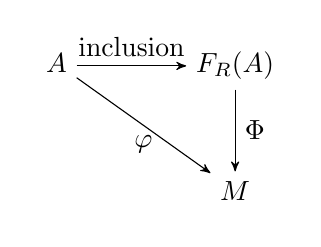
\begin{tikzpicture}
  \matrix (m)
    [
      matrix of math nodes,
      row sep    = 3em,
      column sep = 4em
    ]
    {
	    A & F_R(A) \\
	     & M            \\
    };
  \path
  (m-1-2) edge [->] node [right] {\(\Phi \)} (m-2-2)
    (m-1-1.east |- m-1-2)
    edge [->] node [above] {inclusion} (m-1-2)
      (m-1-1) edge [->] node [below] {$\varphi$} (m-2-2);
\end{tikzpicture}
\end{center}
Furthermore, if \(A = \left\{ a_1,\ldots,a_n \right\} \), then
\begin{align*}
	F_R(A) = Ra_1 \oplus Ra_2 \oplus \ldots \oplus Ra_n \stackrel{R}{\cong} R^{n}
\end{align*}
\end{thm}
This corresponds to the notion of free groups from group theory.

\begin{hw}
	If \(F_R,F_R'\) are free modules on the same set \(A\), there is a unique isomorphism between \(F_R\) and \(F_R'\) which is the identity map on \(A\).\\

	If \(\prescript{}{R}F\) is any free \(R\)-module with basis \(A\), then \(\prescript{}{R}F \cong F_R(A)\).
\end{hw}
If we have a free \(R\)-module with a basis \(A\), the above statement says that we can define \(R\)-module homomorphisms from the free module into other \(R\)-modules by simply specifying how the homomorphism acts on elements of \(A\).\\

The free module \(F_\Z(A)\) is called the \textbf{free abelian group on \(A\)}. If \(A\) is finite, then we say it is of \textbf{rank \(\left| A \right| \)} and is isomorphic to
\begin{align*}
	\Z \oplus \ldots^{n} \oplus \Z.
\end{align*}

%---
%
%diagonalizaton of modules etc
%
%---

\end{document}



\section{Generators and Relations of Modules}
\label{sec:generators_and_relations_of_modules}
\documentclass{memoir}
\usepackage{notestemplate}

%\logo{~/School-Work/Auxiliary-Files/resources/png/logo.png}
%\institute{Rice University}
%\faculty{Faculty of Whatever Sciences}
%\department{Department of Mathematics}
%\title{Class Notes}
%\subtitle{Based on MATH xxx}
%\author{\textit{Author}\\Gabriel \textsc{Gress}}
%\supervisor{Linus \textsc{Torvalds}}
%\context{Well, I was bored...}
%\date{\today}

%\makeindex

\begin{document}

% \maketitle

% Notes taken on 

\begin{defn}[Presentations]
	Let an \(m\times n\) \(R\)-matrix denoted by \(A\) be a homomorphism of \(R\)-modules
	\begin{align*}
		R^{n}\stackrel{A}{\to} R^{m}.
	\end{align*}
	We can denote its image by \(AR^{n}\). We say that the quotient module \(V = R^{m}/ AR^{n}\) is \textbf{presented} by the matrix \(A\). Any isomorphism \(\sigma:R^{m} / AR^{n} \to V\) is a \textbf{presentation} of a module \(V\), of which \(A\) is a \textbf{presentation matrix} for \(V\) if there is such an isomorphism.
\end{defn}

We use the canonical map \(\pi:R^{m}\to V = R^{m} / AR^{n}\) to interpret the quotient module as follows:
\begin{prop}
\(V\) is generated by a set of elements \(B = (v_1,\ldots,v_m)\), the images of the standard basis elements of \(R^{m}\). Furthermore, if \(Y\) is a column vector in \(R^{m}\), the element \(BY\) of \(V\) is zero if and only if \(Y\) is a linear combination of the columns of \(A\), with coefficients in \(R\), if and only if there exists a column vector \(X\) with entries in \(R\) such that \(Y=AX\).
\end{prop}
If a module \(V\) is generated by a set \(B = (v_1,\ldots,v_m)\), we call any element \(Y \in R^{m}\) such that \(BY = 0\) a \textbf{relation vector}, or simply a \textbf{relation} among the generators. A set \(S\) of relations is a \textbf{complete set} if every relation is a linear combination of \(S\) with coefficients in the ring.
\begin{prop}[Theoretical Method of Finding a Presentation]
	First, choose a set of generators \(B = (v_1,\ldots,v_m)\) for \(V\). These generators give a surjective homomorphism \(R^{m}\to V\) that sends a column vector \(Y\) to the linear combination \(BY = v_1y_1+\ldots+v_my_m\). Denote the kernel of the map by \(W\). It is the \textbf{module of relations}; its elements are the relation vectors.\\

	Repeat this procedure, choosing a set of generators \(C = (w_1,\ldots,w_m)\) for \(W\), and define a surjective map \(R^{n}\to W\) using them. Here the generators \(w_j\) are elements of \(R^{m}\), and thus column vectors. Assemble the coordinate vectors \(A_j\) of \(w_j\) into a matrix with \(A_i\) as column \(i\). Then multiplication by \(A\) defines
	\begin{align*}
		R^{n}\to^{A} R^{m}
	\end{align*}
	which sends \(e_j \mapsto A_j = w_j\), as it is the composition of \(R^{n}\to W\) with the inclusion \(W \subset R^{m}\). By construction \(W\) is its image and we denote it by \(AR^{n}\). Because the map \(R^{m}\to V\) is surjective, by the First Isomorphism Theorem, \(V\) is isomorphic to \(R^{m}/W = R^{m}/AR^{n}\). Hence \(V\) is presented by the matrix \(A\).\\

	In short the presentation matrix \(A\) for a module \(V\) is determined by the set of generators for \(V\), and the set of generators for the module of relations \(W\). Assuming the set of generators does not form a basis, the number of generators will be equal to the number of rows of \(A\).
\end{prop}
Note that this relies on the assumption that \(V\) has finite generators. We must also assume that \(W\) has a finite set of generators, which is slightly more problematic.

\begin{prop}[Rules for manipulating \(A\) without changing isomorphism class]
	Let \(A\) be an \(m \times n\) presentation matrix for a module \(V\). The following matrices \(A' \) present the same module \(V\):
	\begin{itemize}
		\item \(A' = Q^{-1}A\), \(Q \in GL_m(R)\)
		\item \(A' = AP\) with \(P \in GL_n(R)\)
		\item \(A'\) is obtained by deleting a column of zeroes
		\item if the \(j\)-th column of \(A\) is \(e_i\), then removing row \(i\) and column \(j\) preserves the presentation
	\end{itemize}
\end{prop}

% \printindex
\end{document}



\section{Modules of Noetherian Rings}
\label{sec:modules_of_Noetherian_rings}
\documentclass{memoir}
\usepackage{notestemplate}

%\logo{~/School-Work/Auxiliary-Files/resources/png/logo.png}
%\institute{Rice University}
%\faculty{Faculty of Whatever Sciences}
%\department{Department of Mathematics}
%\title{Class Notes}
%\subtitle{Based on MATH xxx}
%\author{\textit{Author}\\Gabriel \textsc{Gress}}
%\supervisor{Linus \textsc{Torvalds}}
%\context{Well, I was bored...}
%\date{\today}

%\makeindex

\begin{document}

% \maketitle

% Notes taken on 


\begin{prop}
	The following conditions on an \(R\)-module \(V\) are equivalent:
	\begin{itemize}
		\item Every submodule of \(V\) is finitely generated
		\item There is no infinite strictly increasing chain \(W_1 < W_2 < \ldots\) of submodules of \(V\).
	\end{itemize}
\end{prop}

We formalize this notion via Noetherian rings and modules.

\begin{defn}[Noetherian Modules]
A left \(R\)-module \(\prescript{}{R}M\) is said to be a \textbf{Noetherian \(R\)-module} if it satisfies the ascending chain condition on submodules. That is, for any increasing chain of submodules of \(M\) 
\begin{align*}
	M_1\subset M_2 \subset M_3 \subset \ldots
\end{align*}
there is a positive integer \(m\) such that, for all \(k\geq m\), \(M_k = M_m\).\\

	A ring \(R\) is \textbf{Noetherian} if it is Noetherian as a left module over itself. That is, there are no infinite increasing chains of left ideals of \(R\).
\end{defn}
\begin{cor}
	If \(R\) is Noetherian then every ideal of \(R\) is finitely generated.
\end{cor}

\begin{thm}[Submodules of Noetherian]
	Let \(R\) be a ring and \(\prescript{}{R}M\) a left \(R\)-module. Then the following are equivalent:
	\begin{itemize}
		\item \(M\) is a Noetherian \(R\)-module
		\item Every nonempty set of submodules of \(M\) contains a maximal element under inclusion
		\item Every submodule of \(M\) is finitely generated
	\end{itemize}
\end{thm}
Notice that these conditions also imply that \(R\) is a Noetherian ring, and furthermore that every proper ideal of \(R\) is a maximal ideal.

\begin{cor}
	If \(R\) is a PID then every collection of ideals of \(R\) has a maximal element, and \(R\) is Noetherian.
\end{cor}

\begin{lemma}
	Let \(\varphi:V\to V'\) be a homomorphism of \(R\)-modules.
	\begin{itemize}
		\item If \(V\) is finitely generated and \(\varphi\) is surjective, then \(V'\) is finitely generated.
		\item If the kernal and image of \(\varphi\) are finitely generated, then \(V\) is finitely generated.
		\item Let \(W\) be a submodule of an \(R\)-module \(V\). If both \(W\) and \(\overline{V} = V / W\) are finitely generated, then \(V\) is finitely generated. If \(V\) is finitely generated, so is \(\overline{V}\).
	\end{itemize}
\end{lemma}

\begin{thm}[Hilbert Basis Theorem]
	Let \(R\) be a Noetherian ring. The polynomial ring \(R[x]\) is Noetherian.
\end{thm}

\begin{prop}[Quotients of Noetherian]
	Let \(R\) be a Noetherian ring, and let \(I\) be an ideal of \(R\). Any ring that is isomorphic to the quotient ring \(\overline{R} = R / I\) is Noetherian.
\end{prop}
\begin{cor}
	Let \(P\) be a polynomial ring in a finite number of variables over the integers/field. Any ring \(R\) that is isomorphic to the quotient ring \(P / I\) is Noetherian.
\end{cor}
\begin{lemma}
	Let \(R\) be a ring, let \(I\) be an ideal of the polynomial ring \(R[x]\). The set \(A\) whose elements are the leading coefficients of the nonzero polynomials in \(I\), together with the zero element of \(R\), is an ideal of \(R\), the \textbf{ideal of leading coefficients}.
\end{lemma}



% \printindex
\end{document}


\section{Structure of Abelian Groups}
\label{sec:structure_of_abelian_groups}

\documentclass{memoir}
\usepackage{notestemplate}

%\logo{~/School-Work/Auxiliary-Files/resources/png/logo.png}
%\institute{Rice University}
%\faculty{Faculty of Whatever Sciences}
%\department{Department of Mathematics}
%\title{Class Notes}
%\subtitle{Based on MATH xxx}
%\author{\textit{Author}\\Gabriel \textsc{Gress}}
%\supervisor{Linus \textsc{Torvalds}}
%\context{Well, I was bored...}
%\date{\today}

%\makeindex

\begin{document}

% \maketitle

% Notes taken on 

Recall the fundamental theorem of finitely generated abelian groups.

\begin{thm}[Structure Theorem for Abelian Groups]
	A finitely generated abelian group V is a direct sum of cyclic subgroups \(C_{d_1},\ldots,C_{d_k}\) and a free abelian group \(L\):
	\begin{align*}
		V = C_{d_1}\bigoplus \ldots \bigoplus C_{d_k}\bigoplus L,
	\end{align*}
	where the order \(d_i\) of \(C_{d_i}\) is greater than one, and \(d_i \mid d_{i+1}\) for \(i<k\).
\end{thm}

\begin{thm}[Structure Theorem (Alternate Form)]
	Every finite abelian group is a direct sum of cyclic groups of prime power orders.
\end{thm}
\begin{thm}[Uniqueness for Structure Theorem]
	Suppose that a finite abelian group \(V\) is a direct sum of cyclic groups of prime power orders \(d_j = p_j^{r_k}\). The integers \(d_j\) are uniquely determined by the group \(V\).
\end{thm}

\subsection{Analogues for Polynomial Rings and Linear Operators}
\label{sub:analogues_for_polynomial_rings_and_linear_operators}

\begin{thm}
	Let \(R = F[t]\) be a polynomial ring in one variable over a field \(F\) and let \(A\) be an \(m\times n\) \(R\)-matrix. There are products \(Q,P\) of elementary \(R\)-matrices such that
	\begin{align*}
		A' = Q^{-1}AP
	\end{align*}
	is diagonal, each non-zero diagonal entry \(d_i\) of \(A'\) is a monic polynmial, and \(d_1\mid \ldots\mid d_k\).
\end{thm}

\begin{rmrk}
Let \(M\) be a free cyclic \(R\)-module. Then there is a surjective homomorphism \(\varphi:R\to M\) defined by \(r\mapsto rv\), where \(v\) is the singular generating element in \(M\). The kernel of \(\varphi\) is a submodule of \(R\) and hence an ideal \(I \triangleleft R\). Therefore, \(M\) is isomorphic to the \(R\)-module \(R / I\). When \(R = F[t]\), the ideal \(I\) will be principal.
\end{rmrk}

\begin{thm}[Structure Theorem for Modules over Polynomial Rings]
	Let \(R = F[t]\) be the ring of polynomials in one variable with coefficients in a field \(F\). Let \(V\) be a finitely generated module over \(R\). Then V is a direct sum of cyclic modules \(C_1,C_2,\ldots,C_k\) and a free module \(L\), where \(C_i\) is isomorphic to \(R / (d_i)\), the elements \(d_1,\ldots,d_k\) are monic polynomials of positive degree and satisfy both (but not simultaneously)
\begin{itemize}
	\item \(d_1\mid d_2\mid \ldots\mid d_k\) 
	\item Each \(d_i\) is a power of a monic irreducible polynomial
\end{itemize}
\end{thm}

% \printindex
\end{document}


\section{Tensor Products}
\label{sec:tensors}

\documentclass{memoir}
\usepackage{notestemplate}
\usetikzlibrary{matrix,arrows.meta}

%\logo{~/School-Work/Auxiliary-Files/resources/png/logo.png}
%\institute{Rice University}
%\faculty{Faculty of Whatever Sciences}
%\department{Department of Mathematics}
%\title{Class Notes}
%\subtitle{Based on MATH xxx}
%\author{\textit{Author}\\Gabriel \textsc{Gress}}
%\supervisor{Linus \textsc{Torvalds}}
%\context{Well, I was bored...}
%\date{\today}

%\makeindex

\begin{document}

% \maketitle

% Notes taken on 

The idea of a tensor product of modules \(M,N\) is to form another module in which we can take products \(mn\) of elements \(m \in M\) and \(n \in N\).

\begin{defn}[Ring Extension]
	Let \(R\leq S\). If \(\prescript{}{S}N\) is a left \(S\)-module, then \(N\) can also construct a left \(R\)-module since the elements of \(R\) act on \(N\) by assumption.\\

	More generally, if \(f:R\to S\) is a ring homomorphism from \(R\) into \(S\) with \(f(1_R) = 1_S\), then \(N\) can be considered as an \(R\)-module with \(rn = f(r)n\) for \(r \in R\) and \(n \in N\). We consider \(S\) a \textbf{ring extension of \(R\)} and the resulting \(R\)-module is said to be obtained from \(N\) by \textbf{restriction of scalars} from \(S\) to \(R\).
\end{defn}
One might wonder if the reverse can be done-- taking a ring \(R\) and attempting to extend the scalars to a larger ring. This cannot be done in general-- for example, one can check that \(\Z\) cannot be made into a \(\Q\)-module.\\

However, while \(\Z\) cannot be made into a \(\Q\)-module, it is contained in a \(\Q\)-module (\(\prescript{}{\Q}\Q\)). That is, there is an embedding of the \(\Z\)-module \(\prescript{}{\Z}\Z\) into the \(\Q\)-module \(\prescript{}{\Q}\Q\). This isn't always the case however-- to see this, consider the \(\Z\)-module \(\prescript{}{\Z}N\) where \(N\) is a finite abelian group. One can check that there are no nonzero homomorphisms into any \(\Q\)-module.\\

Our goal will be to construct a module which is the best candidate for which we can embed into.

\begin{defn}[Tensor Product of Modules]
	Let \(\prescript{}{R}N\) be a general \(R\)-module that we wish to embed into some \(S\)-modue. First we will try and define a product of the form \(sn\) for \(s \in S\), \(n \in N\).\\

	We start by considering the free \(\Z\)-module on the set \(S\times N\). This is the collection of all finite commuting sums of elements of the form \((s_i,n_i)\) with no relations imposed on \(sn\). Our \(S\)-module structure requires that we must satisfy the relations
	\begin{align*}
		r_1:& \quad(s_1+s_2)n = s_1n + s_2n \\
		r_2:& \quad s(n_1+n_2) = sn_1 + sn_2\\
		r_3:& \quad (sr)n = s(rn)
	\end{align*}
	for \(s_1,s_2,s \in S\), \(r \in R\), and \(n \in N\). We let \(H\leq N\) be the subgroup given by \(H := \langle r_1,r_2,r_3 \rangle \), that is, all elements of the form above, and consider \(N / H\). We denote this quotient group by \(S \otimes_R N\) and call it the \textbf{tensor module product of \(S\) and \(N\) over \(R\)}. We denote \(s \otimes n\) the coset containing \((s,n)\) in \(S \otimes_R N\) and so we have
	\begin{align*}
		(s_1+s_2) \otimes n = s_1\otimes n + s_2 \otimes n\\
		s \otimes (n_1+n_2) = s\otimes n_1 + s \otimes n_2\\
		sr \otimes n = s \otimes rn.
	\end{align*}
	The elements of \(S \otimes_R N\) are called \textbf{tensors of modules} and can be written as finite sums of \textbf{simple tensors of modules} of the form \(s \otimes n\) with \(s \in S, n \in N\).\\

	Now we give the tensor module product \(S \otimes_R N\) an \(S\)-module action by
	\begin{align*}
		s\left( \sum_{\textrm{finite}} s_i \otimes n_i \right) = \sum_{\textrm{finite}} (ss_i) \otimes n_i.
	\end{align*}
	We call this module \(\prescript{}{S}(S \otimes_R N)\) the \textbf{\(S\)-module obtained by extension of scalars from the \(R\)-module \(N\)}.
\end{defn}
The natural map \(\iota: N \to S \otimes_R N\) defined by \(n\mapsto 1 \otimes n\). Because \(1 \otimes rn = r(1 \otimes n)\), it follows that \(\iota\) is an \(R\)-module homomorphism from \(N\) to \(S \otimes_R N\). It is not injective in general, and so \(S \otimes_R N\) need not contain an isomorphic copy of \(N\).\\

Because the relatons imposed were the minimal relations necessary, one would expect that \(S \otimes_R N\) is the best possible \(S\)-module for a module homomorphism.

\begin{thm}[Universal Property for Tensor Modules]
	Let \(R\leq S\), let \(\prescript{}{R}N\) be a left \(R\)-module and let \(\iota: N \to S \otimes_R N\) be the \(R\)-module homomorphism defined by \(\iota(n) = 1 \otimes n\). Suppose that \(\prescript{}{S}L\) is an arbitrary left \(S\)-module and \(\varphi :N \to L\) is an \(R\)-module homomorphism from \(N\) to \(L\). Then there is a unique \(S\)-module homomorphism \(\Phi :S \otimes_R N \to L\) such that \(\varphi = \Phi \circ \iota \) and the diagram commutes:
\begin{center}
			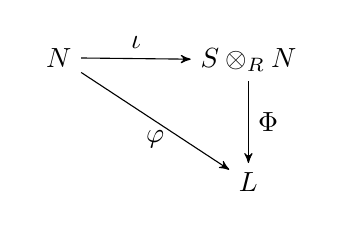
\begin{tikzpicture}
  \matrix (m)
    [
      matrix of math nodes,
      row sep    = 3em,
      column sep = 4em
    ]
    {
	    N & S \otimes_R N \\
	     & L            \\
    };
  \path
  (m-1-2) edge [->] node [right] {\(\Phi \)} (m-2-2)
    (m-1-1) edge [->] node [above] {\(\iota\)} (m-1-2)
      (m-1-1) edge [->] node [below] {$\varphi$} (m-2-2);
\end{tikzpicture}
\end{center}
Conversely, if \(\Phi :S \otimes_R N \to L\) is an \(S\)-module homomorphism then \(\varphi  = \Phi \circ \iota\) is an \(R\)-module homomorphism from \(N\) to \(L\).
\end{thm}

\begin{cor}
	Let \(\iota:N \to S \otimes_R N\) be the \(R\)-module homomorphism from the universal property of free modules. Then \(N / \textrm{Ker}\iota\) is the unique largest quotient of \(N\) that can be embedded in any \(S\)-module.\\

	In particular, \(N\) can be embedded as an \(R\)-submodule of some left \(S\)-module if and only if \(\iota\) is injective.
\end{cor}

\begin{exmp}
	
\end{exmp}


\subsection{General Tensor Product}
\label{sub:general_tensor_product}

Notice that forming \(S\otimes_R N\) as an abelian group only required \(S_R\) to be a right \(R\)-module and \(\prescript{}{R}N\) a left \(R\)-module. We can construct an abelian group \(M \otimes_R N\) for any right \(R\)-module \(M_R\) and any left \(R\)-module \(\prescript{}{R}N\).\\

The \(S\)-module structure on \(\prescript{}{S}{(S \otimes_R N)}\) required only a left \(S\)-module structure on \(\prescript{}{S}S\) and the compatibility relation
\begin{align*}
	s'(^2) = (s's)r.
\end{align*}

\begin{defn}[Tensor]
	Let \(\prescript{}{R}N\) be a left \(R\)-module and \(M_R\) a right \(R\)-module. We obtain an abelian group by quotient of the free \(\Z\)-module on \(M\times N\) by the subgroup \(H = \langle r_1,r_2,r_3 \rangle \), where
	\begin{align*}
		r_1:& \quad (m_1+m_2,n) = (m_1,n) + (m_2,n)\\
		r_2:& \quad (m, n_1+n_2) = (m,n_1) + (m,n_2)\\
		r_3:& \quad (mr,n) = (m,rn)
	\end{align*}
	for \(m,m_1,m_2 \in M\), \(n,n_1,n_2 \in N\), and \(r \in R\). We denote this by
	\begin{align*}
		M \otimes_R N := \prescript{}{\Z}(M \times N) / \langle r_1,r_2,r_3 \rangle 
	\end{align*}
	and call it the \textbf{tensor product of \(M\) and \(N\) over \(R\)}. The elements of \(M \otimes_R N\) are called \textbf{tensors}, and the coset \(m \otimes n \in M \otimes_R N\) is called a \textbf{simple tensor}. Every tensor can be written (non-uniquely) as a finite sum of simple tensors.
\end{defn}
Keep in mind that \(m \otimes n\) are cosets and not elements directly-- so caution must be used when defining maps on tensor products. That is, one needs to check that a map is well-defined on the entirety of a coset.\\

Furthermore, caution must be exercised when comparing tensor products. For example, if \(M \leq M'\), we can have \(m \otimes n = 0\) in \(M' \otimes_R N\) but \(m \otimes n \neq 0\) in \(M \otimes_R N\). This essentially captures the notion that when more elements are included, the cosets will change. Hence there is no reason to expect \(M \otimes_R N \leq M' \otimes_R N\).

\begin{defn}
	Let \(M_R\) be a right \(R\)-module, \(\prescript{}{R}N\) a left \(R\)-module, and \(L\) an abelian group. A map \(\varphi :M\times N \to L\) is called \textbf{\(R\)-balanced} or \textbf{middle linear with respect to \(R\)} if
	\begin{align*}
		\varphi (m_1+m_2,n) &= \varphi(m_1,n) + \varphi (m_2,n)\\
		\varphi (m,n_1+n_2) &= \varphi (m,n_1) + \varphi (m,n_2)\\
		\varphi (m,rn) &= \varphi (mr,n)
	\end{align*}
	for all \(m,m_1,m_2 \in M\), \(n,n_1,n_2 \in N\) and \(r \in R\).
\end{defn}
We can define a map \(\iota:M\times N \to M \otimes_R N\) with \(\iota(m,n) = m \otimes n\). This map is not a group homomorphism but it is in fact \(R\)-balanced.

\begin{thm}[Universal Property of Tensor Products]
	Let \(R\) be a ring, \(M_R\) a right \(R\)-module, and \(\prescript{}{R}N\) a left \(R\)-module. Let \(M \otimes_R N\) be the tensor product of \(M\) and \(N\) over \(R\) and let \(\iota: M \times N \to M \otimes_R N\) be the \(R\)-balanced map defined by \(\iota(m,n) = m \otimes n\). Then for any group homomorphism \(\Phi :M \otimes_R N \to L\) to an abelian group \(L\), the composite map
	\begin{align*}
		\varphi = \Phi \circ \iota
	\end{align*}
	is an \(R\)-balanced map from \(M \times N \to L\). Conversely, if \(L\) is an abelian group and \(\varphi :M \times N \to L\) is any \(R\)-balanced map, then there is a unique group homomorphism \(\Phi: M \otimes_R N \to L\) such that \(\varphi  = \Phi \circ \iota\).\\

	In other words, there is a correspondence between \(\varphi \) and \(\Phi \) by the commutative diagram:
\begin{center}
			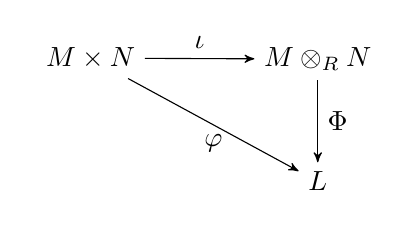
\begin{tikzpicture}
  \matrix (m)
    [
      matrix of math nodes,
      row sep    = 3em,
      column sep = 4em
    ]
    {
	    M \times N & M \otimes_R N \\
	     & L            \\
    };
  \path
  (m-1-2) edge [->] node [right] {\(\Phi \)} (m-2-2)
    (m-1-1) edge [->] node [above] {\(\iota\)} (m-1-2)
      (m-1-1) edge [->] node [below] {$\varphi$} (m-2-2);
\end{tikzpicture}
\end{center}
and this correspondence establishes a bijection between \(R\)-balanced maps and group homomorphisms, by the bijection between \(\varphi \) and \(\Phi \).
\end{thm}

\begin{cor}
	Suppose \(D\) is an abelian group and \(\iota':M \times N \to D\) is an \(R\)-balanced map such that
	\begin{itemize}
		\item \(D = \langle \textrm{Im}(\iota')\rangle \) 
		\item every \(R\)-balanced map defined on \(M\times N\) factors through \(\iota'\)
	\end{itemize}
	Then there is an isomorphism \(f: M \otimes_R N \cong D\) of abelian groups with \(\iota' = f \circ \iota\)
\end{cor}

Now we'd like to give this abelian group a module structure. We simply need to impose a compatibility structure on \(M\) to obtain this.

\begin{defn}
	Let \(R,S\) be rings. An abelian group \(M\) induces a \textbf{\((S,R)\)-bimodule} if \(M\) forms a left \(S\)-module, a right \(R\)-module, and \(s(mr) = (sm)r\) for all \(s \in S, r \in R, m \in M\).
\end{defn}

\begin{exmp}
	Let \(R\) be a commutative ring. A left \(R\)-module \(\prescript{}{R}M\) can always be given the structure of a right \(R\)-module by simply defining \(mr = rm\), and hence \(M\) becomes a \((R,R)\)-bimodule. We call this the \textbf{standard} \(R\)-module structure on \(M\).
\end{exmp}
Notice that if \(N\) has a left \(R\)-module structure and \(M\) a \((S,R)\)-bimodule structure, then we have once again
\begin{align*}
	s \left( \sum_{\textrm{finite}} m_i \otimes n_i \right) = \sum_{\textrm{finite}} (sm_i) \otimes n_i
\end{align*}
and hence there is a well-defined action of \(S\) so that \(M \otimes_R N\) can be considered a left \(S\)-module. It follows that for fixed \(s\), \((m,n)\mapsto sm \otimes n\) is an \(R\)-balanced map, and hence there is a well-defined group homomorphism \(\lambda_s:M\otimes_R N \to M \otimes_R N\) that satisfies \(\lambda_s(m \otimes n) = sm \otimes n\).\\

A special case we might encounter is when \(M,N\) are left modules over a commutative ring \(R\), and \(S = R\). Then the standard \(R\)-module structure on \(M\) gives \(M\) the structure of an \((R,R)\)-bimodule and hence \(M \otimes_R N\) always has the structure of a left \(R\)-module.

\begin{defn}
	Let \(R\) be a commutative ring and let \(M,N,L\) be left \(R\)-modules. The map \(\varphi : M \times N \to L\) is called \textbf{\(R\)-bilinear} if it is \(R\)-linear in every factor:
	\begin{align*}
		\varphi (r_1m_1+r_2m_2,n) &= r_1 \varphi (m_1,n) + r_2 \varphi (m_2,n)\\
		\varphi (m,r_1n_1 + r_2n_2) = r_1 \varphi (m,n_1) + r_2 \varphi (m,n_2)
	\end{align*}
	for all \(m, m_1, m_2 \in M\), \(n,n_1,n_2 \in N\), and \(r_1,r_2 \in R\).
\end{defn}

\begin{cor}
	Suppose \(R\) is a commutative ring, and \(M,N\) two left \(R\)-modules. Let \(M \otimes_R N\) be the tensor product of \(M\) and \(N\) over \(R\), where \(M\) is given the standard \(R\)-module structure. Then \(M \otimes_R N\) is a left \(R\)-module with
	\begin{align*}
		r(m \otimes n) = (rm) \otimes n = (mr) \otimes n = m \otimes (rn)
	\end{align*}
	and the map \(\iota:M \times N \to M \otimes_R N\) with \(\iota(m,n) = m \otimes n\) is an \(R\)-bilinear map. If \(L\) is any left \(R\)-module then there is a bijection between \(R\)-bilinear maps and \(R\)-module homomorphisms induced by the bijection between \(\varphi: M\times N \to L \) and \(\Phi: M \otimes_R N \to L \) via the commutative diagram:
\begin{center}
			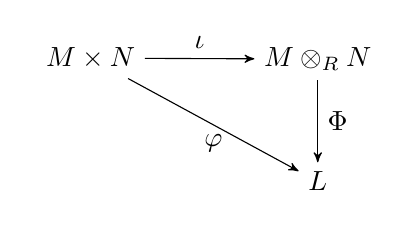
\begin{tikzpicture}
  \matrix (m)
    [
      matrix of math nodes,
      row sep    = 3em,
      column sep = 4em
    ]
    {
	    M \times N & M \otimes_R N \\
	     & L            \\
    };
  \path
  (m-1-2) edge [->] node [right] {\(\Phi \)} (m-2-2)
    (m-1-1) edge [->] node [above] {\(\iota\)} (m-1-2)
      (m-1-1) edge [->] node [below] {$\varphi$} (m-2-2);
\end{tikzpicture}
\end{center}
\end{cor}

\begin{exmp}
		
\end{exmp}

\begin{thm}[Tensor Product of Homomorphisms]
	Let \(M, M'\) be right \(R\)-modules, let \(N,N'\) be left \(R\)-modules. Suppose \(\varphi :M \to M'\) and \(\psi : N \to N'\) are \(R\)-module homomorphisms. Then there is a unique group homomorphism denoted by \(\varphi  \otimes \psi \) given by
	\begin{align*}
		\varphi \otimes \psi : M \otimes_R N \to M' \otimes_R N'\\
		(\varphi \otimes \psi )(m \otimes n) = \varphi (m) \otimes \psi (n)
	\end{align*}
	for all \(m \in M\) and \(n \in N\).\\

	If \(M,M'\) are \((S,R)\)-bimodules for some ring \(S\), and \(\varphi \) is also an \(S\)-module homomorphism, then \(\varphi \otimes \psi \) is a homomorphism of left \(S\)-modules. Hence if \(R\) is commutative then \(\varphi \otimes \psi \) is always an \(R\)-module homomorphism for the standard \(R\)-module structures.
\end{thm}
Notice that the uniqueness conditions tells us that if \(\lambda :M' \to M''\) and \(\mu : N' \to N''\) are \(R\)-module homomorphisms, then
\begin{align*}
	(\lambda \otimes u ) \circ (\varphi  \otimes \psi ) = (\lambda \circ \varphi ) \otimes (\mu  \otimes \psi ).
\end{align*}
In fact, we can use this idea to extend the tensor product into an \(n\)-fold tensor product.

\begin{thm}
	Suppose \(M\) is a right \(R\)-module, \(N\) is an \((R,T)\)-bimodule, and \(L\) is a left \(T\)-module. Then there is a unique isomorphism
	\begin{align*}
		(M \otimes_R N) \otimes_T L \cong M \otimes_R (N \otimes_T L)
	\end{align*}
	of abelian groups such that
	\begin{align*}
		(m \otimes_R n) \otimes l \mapsto m \otimes_R(n \otimes_R l).
	\end{align*}
	If \(M\) is an \((S,R)\)-bimodule, then this is an isomorphism of \(S\)-modules.
\end{thm}

\begin{cor}
	Let \(R\) be a commutative ring and \(M,N,L\) form left \(R\)-modules. Then
	\begin{align*}
		(M \otimes_R N) \otimes_R L \cong M \otimes_R(N \otimes_R L)
	\end{align*}
\end{cor}
Of course, it will be useful to use the natural extension of a bilinear map.

\begin{defn}
	Let \(R\) be a commutative ring and  let \(M_1,M_2,\ldots,M_n\) and \(L\) form \(R\)-modules with the standard \(R\)-module structures. A map \(\varphi : M_1 \times  \ldots \times M_n \to L\) is called \textbf{\(n\)-multilinear over \(R\)} if it is an \(R\)-module homomorphism in each component:
	\begin{align*}
		\varphi (m_1,\ldots,m_{i-1},rm_i + r'm'_i, m_{i+1},\ldots,m_n) = r \varphi(m_1,\ldots,m_i,\ldots,m_n) + r' \varphi (m_1,\ldots,m_i', \ldots, m_n)
	\end{align*}
\end{defn}
Hence we can define an \(n\)-fold tensor product by iterating the tensor product of pairs of modules.

\begin{cor}
	Let \(R\) be a commutative ring and let \(M_1,\ldots,M_n,L\) be \(R\)-modules. Let \(M_1 \otimes_R M_{2} \otimes_R \ldots \otimes_R M_n\) be the sequence of tensor products of pairs of these modules and let
	\begin{align*}
		\iota:M_1\times \ldots \times M_n \to M_1 \otimes_R \ldots \otimes_R M_n\\
		\iota(m_1,\ldots,m_n) = m_1 \otimes_R \ldots \otimes_R m_n.
	\end{align*}
	Then for every \(R\)-module homomorphism \(\Phi : M_1 \otimes_R \ldots \otimes_R M_n \to L\) the map \(\varphi = \Phi \circ \iota\) is \(n\)-multilinear from \(M_1\times \ldots\times M_n\to L\).\\

	If \(\varphi :M_1\times \ldots\times M_n \to L\) is an \(n\)-multilinear map then there is a unique \(R\)-module homomorphism \(\Phi :M_1 \otimes_R \ldots \otimes_R M_n \to L\) such that \(\varphi  = \Phi \circ \iota\). This bijection induces a bijection between \(n\)-multilinear maps and \(R\)-module homomorphisms for which the following diagram commutes:
\begin{center}
			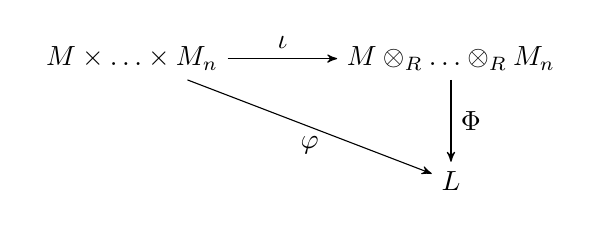
\begin{tikzpicture}
  \matrix (m)
    [
      matrix of math nodes,
      row sep    = 3em,
      column sep = 4em
    ]
    {
	    M \times \ldots \times M_n & M \otimes_R \ldots \otimes_R M_n \\
	     & L            \\
    };
  \path
  (m-1-2) edge [->] node [right] {\(\Phi \)} (m-2-2)
    (m-1-1) edge [->] node [above] {\(\iota\)} (m-1-2)
      (m-1-1) edge [->] node [below] {$\varphi$} (m-2-2);
\end{tikzpicture}
\end{center}
\end{cor}

We once again have a containment condition.

\begin{thm}[Tensor Products of Direct Sums]
	Let \(M, M'\) be right \(R\)-modules and let \(N, N'\) be left \(R\)-modules. Then there are unique group isomorphisms
	\begin{align*}
		(M \oplus M') \otimes_R N \cong (M \otimes_R N) \oplus (M' \otimes_R N)\\
		M \otimes_R (N \oplus N') \cong (M \otimes_R N) \oplus (M \otimes_R N')\\
		(m,m') \otimes n \mapsto (m \otimes n, m' \otimes n)\\
		m \otimes(n,n') \mapsto (m \otimes n, m \otimes n').
	\end{align*}
	If \(M,M'\) are also \((S,R)\)-bimodules, then these are isomorphisms of left \(S\)-modules. In particular, if \(R\) is commutative, these are isomorphisms of \(R\)-modules.
\end{thm}
Of course, this theorem extends inductively to any finite direct sum of \(R\)-modules (in fact any arbitrary direct sums). In essense, tensor products commute with direct sums.

\begin{cor}
	The module obtained from the free \(R\)-module \(N \cong \prescript{}{R}R^{n}\) by extension of scalars from \(R\) to \(S\) is the free \(S\)-module \(\prescript{}{S}S^{n}\):
	\begin{align*}
		S \otimes_R R^{n} \cong S^{n}
	\end{align*}
as left \(S\)-modules.
\end{cor}

\begin{cor}
	Let \(R\) be a commutative ring and let \(M \cong R^{s}\), \(N \cong R^{t}\) form free \(R\)-modules with bases \(m_1,\ldots,m_s\) and \(n_1,\ldots,n_t\) respectively.  Then \(M \otimes_R N\) forms a free \(R\)-module of rank \(st\) with basis \(m_i \otimes n_j\), \(1\leq i\leq s\) and \(1\leq j\leq t\), so that:
	\begin{align*}
		R^{s} \otimes_R R^{t} \cong R^{st}.
	\end{align*}
\end{cor}

\begin{rmrk}
	The tensor product of two free modules of arbitrary rank over a commutative ring is free.
\end{rmrk}

\begin{prop}
	Suppose \(R\) is a commutative ring and \(M,N\) form left \(R\)-modules via the standard \(R\)-module structures. Then there is a unique \(R\)-module isomorphism
	\begin{align*}
		M \otimes_R N \cong N \otimes_R M\\
		m \otimes n \mapsto n \otimes m
	\end{align*}
\end{prop}
One might think that if \(M=N\), the above conditions are not necessary, but in fact it is not the case. Some tensors do have the property that \(a \otimes b = b \otimes a\) for \(a,b \in M\), which we refer to as symmetric tensors, to be studied later.

\begin{prop}
	Let \(R\) be a commutative ring and let \(A,B\) be \(R\)-algebras. Then the multiplication
	\begin{align*}
		(a \otimes b) (a' \otimes b') = a a' \otimes b b'
	\end{align*} is well-defined and makes \(A\otimes_R B\) into an \(R\)-algebra.
\end{prop}

\begin{exmp}
	
\end{exmp}

% \printindex
\end{document}


\section{Exact Sequences}
\label{sec:exact_sequences}

\documentclass{memoir}
\usepackage{notestemplate}
\usetikzlibrary{arrows,chains,matrix,positioning,scopes}

\makeatletter
\tikzset{join/.code=\tikzset{after node path={%
\ifx\tikzchainprevious\pgfutil@empty\else(\tikzchainprevious)%
edge[every join]#1(\tikzchaincurrent)\fi}}}
\makeatother

\tikzset{>=stealth',every on chain/.append style={join},
         every join/.style={->}}

%\logo{~/School-Work/Auxiliary-Files/resources/png/logo.png}
%\institute{Rice University}
%\faculty{Faculty of Whatever Sciences}
%\department{Department of Mathematics}
%\title{Class Notes}
%\subtitle{Based on MATH xxx}
%\author{\textit{Author}\\Gabriel \textsc{Gress}}
%\supervisor{Linus \textsc{Torvalds}}
%\context{Well, I was bored...}
%\date{\today}

%\makeindex

\begin{document}

% \maketitle

% Notes taken on 06/08/21

Consider modules \(A,C\). One question worth exploring is if there exists a module \(B\) such that \(A / B \cong C\); that is, \(B\) is an extension of \(C\) by \(A\). The tools we develop to understand this question are exact sequences. If \(A\) is isomorphic to a submodule of \(B \), there is an injective homomorphism from \(A\) to \(B\). And if \(C\) is isomorphic to the quotient, then there is a surjective homomorphism from \(B\) to \(C\). This will give us a chain
\begin{align*}
	A \to B \to C
\end{align*}
where the homomorphisms are compatible with. We formalize this idea via exact sequences.

\begin{defn}[Exact Sequences]
	Let \(\alpha ,\beta \) be homomorphisms so that
	\begin{align*}
		X \to^{\alpha } Y \to^{\beta }Z.
	\end{align*}
	If \(\textrm{Im}(\alpha ) = \textrm{Ker}(\beta )\), then we say the pair of homomorphisms are \textbf{exact}.\\

	A sequence of homomorphisms
	\begin{align*}
		\ldots \to X_{n-1} \to X_n \to X_{n+1} \to \ldots
	\end{align*}
	is said to be an \textbf{exact sequence} if it is exact at every \(X_n\) between a pair of homomorphisms.
\end{defn}
Hence, our goal is to see whether we can form an exact sequence \(A\to B\to C\). Our notions of injectivity and surjectivity correspond exactly to the notions of exactness.
\begin{prop}
	Let \(A,B,C\) form \(R\)-modules over some ring \(R\). Then the sequence
	\begin{align*}
		0 \to A \to^{\psi }B
	\end{align*}
	is exact at \(A\) if and only if \(\psi \) is injective. Likewise, the sequence
	\begin{align*}
		B \to^{\varphi }\to C \to 0
	\end{align*}
	is exact at \(C\) if and only if \(\varphi \) is surjective.
\end{prop}
Combining the two ideas, the sequence
\begin{align*}
	0 \to A \to^{\psi }B \to^{\varphi }C \to 0
\end{align*}
is exact if and only if \(\psi \) is injective, \(\varphi \) is surjective, and \(\textrm{Im}(\psi ) = \textrm{Ker}(\varphi )\).

\begin{defn}
	An exact sequence of the form
	\begin{align*}
		0 \to A \to^{\psi }B \to^{\varphi }C \to 0
	\end{align*}
	is called an \textbf{short exact sequence}.
\end{defn}
Our goal then is to determine if two modules admit a short exact sequence, and if so, how many.\\

Notice that any exact sequence can be written as a succession of short exact sequences. For example, if
\begin{align*}
	X \to^{\alpha }Y \to^{\beta }Z
\end{align*}
is exact at \(Y\), then equivalently
\begin{align*}
	0 \to \alpha (X) \to Y \to Y / \textrm{Ker}(\beta ) \to 0
\end{align*}
is a short exact sequence.

\begin{exmp}
	
\end{exmp}

For fixed \(A,C\), there can be many extensions of \(C\) by  \(A\). Hence, we need to determine a notion of a homomorphism to distinguish exact sequences.

\begin{defn}[Homomorphism of Short Exact Sequences]
	Let
	\begin{align*}
		0 \to A \to B \to C \to 0\\
		0 \to A' \to B' \to C' \to 0
	\end{align*}
	be two short exact sequences of modules. A \textbf{homomorphism of short exact sequences} is a collection of module homomorphisms \(\alpha ,\beta ,\gamma \) such that the following diagram commutes:
\begin{center}
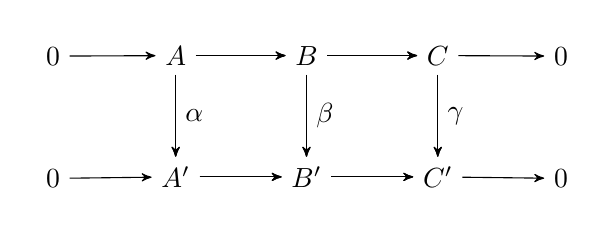
\begin{tikzpicture}
  \matrix (m) [matrix of math nodes, row sep=3em, column sep=3em]
    { 0 & A  & B  & C  & 0 \\
      0 & A' & B' & C' & 0 \\ };
  { [start chain] \chainin (m-1-1);
    \chainin (m-1-2);
    { [start branch=A] \chainin (m-2-2)
        [join={node[right] {$\alpha $}}];}
    \chainin (m-1-3) [join={node[above] {}}];
    { [start branch=B] \chainin (m-2-3)
        [join={node[right] {$\beta $}}];}
    \chainin (m-1-4) [join={node[above] {}}];
    { [start branch=C] \chainin (m-2-4)
        [join={node[right] {$\gamma $}}];}
    \chainin (m-1-5); }
  { [start chain] \chainin (m-2-1);
    \chainin (m-2-2);
    \chainin (m-2-3) [join={node[above] {}}];
    \chainin (m-2-4) [join={node[above] {}}];
    \chainin (m-2-5); }
\end{tikzpicture}
\end{center}
This is an \textbf{isomorphism of short exact sequences} if \(\alpha ,\beta ,\gamma \) are isomorphisms in which case the extensions \(B,B'\) are \textbf{isomorphic extensions}.\\

The two exact sequences are called \textbf{equivalent} if \(A = A'\), \(C = C'\), and there is an isomorphism between them where  \(\alpha ,\gamma \) are identity. In this case \(B\) and \(B'\) are \textbf{equivalent extensions}.
\end{defn}
Equivalency by extensions is stronger than just \(R\)-module isomorphisms between \(B\) and \(B'\)-- it tells us tat there is an \(R\)-module isomorphism between \(B\) and \(B'\) that restricts to an isomorphism from \(A\) to \(A'\) and induces an isomorphism on the quotients by \(C\) and \(C'\).

\begin{exmp}
	
\end{exmp}

\begin{prop}[Short Five Lemma]
	Let \(\alpha ,\beta ,\gamma \) be a homomorphism of short exact sequences
\begin{center}
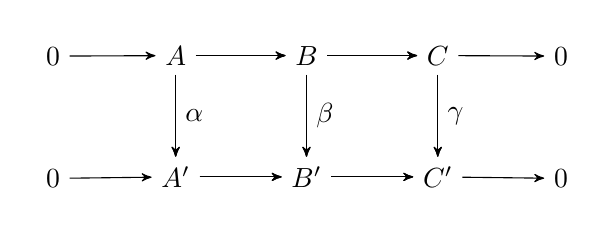
\begin{tikzpicture}
  \matrix (m) [matrix of math nodes, row sep=3em, column sep=3em]
    { 0 & A  & B  & C  & 0 \\
      0 & A' & B' & C' & 0 \\ };
  { [start chain] \chainin (m-1-1);
    \chainin (m-1-2);
    { [start branch=A] \chainin (m-2-2)
        [join={node[right] {$\alpha $}}];}
    \chainin (m-1-3) [join={node[above] {}}];
    { [start branch=B] \chainin (m-2-3)
        [join={node[right] {$\beta $}}];}
    \chainin (m-1-4) [join={node[above] {}}];
    { [start branch=C] \chainin (m-2-4)
        [join={node[right] {$\gamma $}}];}
    \chainin (m-1-5); }
  { [start chain] \chainin (m-2-1);
    \chainin (m-2-2);
    \chainin (m-2-3) [join={node[above] {}}];
    \chainin (m-2-4) [join={node[above] {}}];
    \chainin (m-2-5); }
\end{tikzpicture}
\end{center}
\begin{itemize}
	\item If \(\alpha ,\gamma \) are injective then so is \(\beta \) 
	\item If \(\alpha ,\gamma \) are surjective then so is \(\beta \) 
	\item If \(\alpha ,\gamma \) are isomorphisms then so is \(\beta \)
\end{itemize}
\end{prop}
These results also hold for short exact sequences of groups.

\begin{proof}[Proof of Short Five Lemma]
	
\end{proof}
There is always at least one extension of a module \(C\) by \(A\) given by \(B = A \oplus C\).

\begin{defn}
	Let \(R\) be a ring and let
	\begin{align*}
		0 \to A \to^{\psi }B \to^{\varphi }C \to 0
	\end{align*}
	be a short exact sequence of \(R\)-modules. We say the sequence is \textbf{split} if there is an \(R\)-module complement to \(\psi (A)\) in \(B\). If this holds, then \(B = A \oplus C\) up to isomorphism by
	\begin{align*}
		B = \psi (A) \oplus C'
	\end{align*}
	for some submodile \(C'\), where \(\varphi (C') \cong C\).\\

	We say \(B\) is a \textbf{split extension of \(C\) by \(A\)}.
\end{defn}
This is really just the question of existence of a complement to \(\psi (A)\) in \(B\) that is isomorphic by \(\varphi \) to \(C\).

\begin{prop}
	The short exact sequence
	\begin{align*}
		0 \to A \to^{\psi }B \to^{\varphi }C \to 0
	\end{align*}
	of \(R\)-modules is split if and only if there is an \(R\)-module homomorphism \(\mu :C \to B\) such that \(\varphi \circ \mu \cong \textrm{Id}_C\).\\

	Any set map \(\mu :C\to B\) such that \(\varphi \circ \mu = \textrm{Id}_C\) is called a \textbf{section} of \(\varphi \). If \(\mu \) is a homomorphism, then \(\mu \) is called a \textbf{splitting homomorphism} for the sequence.
\end{prop}
A section of \(\varphi \) is merely a choice of coset representative in \(B\) for \(B / \textrm{Ker}\varphi  \cong C\). A section is a homomorphism if this set of coset representatives forms a submodule, in which case this submodule gives a complement to \(\psi (A)\) in \(B\).

\begin{exmp}
	
\end{exmp}

\begin{prop}
	Let
	\begin{align*}
		0 \to A \to^{\psi }B \to^{\varphi }C \to 0
	\end{align*}
	be a short exact sequence of modules. Then \(B = \psi (A) \oplus C'\) for some submodule \(C'\) of \(B\) with \(\varphi (C') \cong C\) if and only if there is a homomorphism \(\lambda :B\to A\) such that \(\lambda \circ \psi = \textrm{Id}_A\) .
\end{prop}
For groups, this is a stronger notion. The existence of a splitting homomorphism on the left end of the sequence gives that the extension group is a direct product (instead of a semidirect product). Of course, in modules there is no distinction as the underlying groups are abelian.

\subsection{Projective Modules}
\label{sub:projective_modules}

Let \(R\) be a ring and suppose that \(\prescript{}{R}M\) is an extension of \(N\) by \(L\), so that
\begin{align*}
	0 \to L \to^{\psi }M \to^{\varphi }N \to 0.
\end{align*}
If another \(R\)-module has an \(R\)-module homomorphism into \(L\) or \(N\), can it extend to a homomorphism to \(M\)?\\

We can see directly that if \(f \in \textrm{Hom}_R(D,L)\) then \(f' = \psi \circ f\) is an \(R\)-module homomorphism from \(D\) to \(M\):
\begin{align*}
	\psi': \textrm{Hom}_R(D,L) \to \textrm{Hom}_R(D,M)\\
	f \mapsto f' = \psi \circ f.
\end{align*}

\begin{prop}
	Let \(D,L,\) and \(M\) form \(R\)-modules and let \(\psi :L \to M\) be an \(R\)-module homomorphism. Then the map
	\begin{align*}
		\psi': \textrm{Hom}_R(D,L) &\to \textrm{Hom}_R(D,M)\\
		f &\mapsto f' = \psi \circ f
	\end{align*}
	is a homomorphism of abelian groups. If \(\psi \) is injective, then \(\psi '\) is injective. Hence, if
	\begin{align*}
		0 \to L \to^{\psi }M
	\end{align*} is exact, then
	\begin{align*}
		0 \to \textrm{Hom}_R(D,L) \to^{\psi '} \textrm{Hom}_R(D,M)
	\end{align*}
	is exact.
\end{prop}

Unfortunately, if there is an \(R\)-module homomorphism \(f:D \to N\), it isn't always the case that \(f\) \textbf{lifts} to an \(R\)-module homomorphism \(f:D\to M\) by
\begin{align*}
	\varphi ': \textrm{Hom}_R(D,M) &\to \textrm{Hom}_R(D,N)\\
	F &\mapsto F' = \varphi \circ F
\end{align*}
This only holds if and only if \(f\) is in the image of \(\varphi '\).

\begin{exmp}
	
\end{exmp}

\begin{thm}
	Let \(D,L,M,N\) form \(R\)-modules. If
	\begin{align*}
		0 \to L \to^{\psi }M \to^{\varphi }N \to 0
	\end{align*}
	is exact, then
	\begin{align*}
		0 \to \textrm{Hom}_R(D,L) \to^{\psi '} \textrm{Hom}_R(D,M) \to^{\varphi '} \textrm{Hom}_R(D,N)
	\end{align*}
	is exact.\\

	A homomorphism \(f:D\to N\) lifts to a homomorphism \(F:D\to M\) if and only if \(f \in \textrm{Hom}_R(D,N)\) is in the image of \(\varphi '\). In general \(\varphi '\) is surjective if and only if every homomorphism from \(D\) to \(N\) lifts to a homomorphism from \(D\) to \(M\), in which case the sequence above extends to a short exact sequence.\\

	The sequence above is exact for all \(R\)-modules \(D\) if and only if
	\begin{align*}
		0 \to L \to^{\psi }M \to^{\varphi }N
	\end{align*}
	is exact.
\end{thm}
Hence, by the theorem, the sequence
\begin{align*}
	0 \to \textrm{Hom}_R(D,L) \to^{\psi '}\textrm{Hom}_R(D,M) \to^{\varphi '} \textrm{Hom}_R(D,N) \to 0
\end{align*}
is in general not a short exact sequence, as \(\varphi '\) may not be surjective. In fact, this sequence is exact if and only if there is a bijection between homomorphisms \(F:D \to M\) and \(g:D\to L\), \(f:D\to N\) where
\begin{align*}
	F\mid_{\varphi (L)} = \psi'(g)\\
	f = \varphi'(F).
\end{align*}
Notice that if the original sequence is spit exact, then the sequence of homomorphisms is also split exact.
\begin{prop}
	Let \(D,L,N\) form \(R\)-modules. Then
	\begin{align*}
		\textrm{Hom}_R(D,L\oplus N) \cong \textrm{Hom}_R(D,L) \oplus \textrm{Hom}_R(D,N)\\
		\textrm{Hom}_R(L \oplus N, D) \cong \textrm{Hom}_R(L,D) \oplus \textrm{Hom}_R(N,D)
	\end{align*}
\end{prop}
Of course this extends by induction to any finite direct sum of \(R\)-modules. In other words, the group of module homomorphisms commute with dfinite direct sums in either variable.

\begin{rmrk}
	For infinite direct sums, this does not always hold. If \(L \oplus N\) is replaced by an arbitrary direct sum, and the direct sum on the right hand side is replaced by a direct product, then
	\begin{align*}
		\textrm{Hom}_R(D,L\oplus \left\{ N_i \right\}_{i \in I}) \cong \textrm{Hom}_R(D,L) \otimes \left\{ \textrm{Hom}_R(D,N_i) \right\}_{i \in I} 
	\end{align*}
	holds. The second part must be translated into
	\begin{align*}
		\textrm{Hom}_R(L \otimes \left\{ N_i \right\}_{i \in I},D) \cong \textrm{Hom}_R(L,D) \otimes \left\{ \textrm{Hom}_R(N_i,D) \right\}_{i \in I}
	\end{align*}
\end{rmrk}

Hence, a split short exact sequence of \(R\)-modules induces a split short exact sequence of abelian groups for every \(R\)-module \(D\). In fact, the converse holds:
\begin{hw}
	Prove that if
	\begin{align*}
		0 \to \textrm{Hom}_R(D,L) \to^{\psi '} \textrm{Hom}_R(D,M) \to^{\varphi'} \textrm{Hom}_R(D,N) \to 0
	\end{align*} is exact for every \(R\)-module \(D\), then
	\begin{align*}
		0 \to L \to^{\psi }M \to^{\varphi }N \to 0
	\end{align*}
	is a split short exact sequence.\\

	This implies that if the original homomorphism sequence is exact for every \(D\), then it is in fact split exact for every \(D\).
\end{hw}

\begin{prop}
	Let \(P\) be an \(R\)-module. Then the following are equivalent:
	\begin{itemize}
		\item Let \(L,M,N\) form \(R\)-modules. If
			\begin{align*}
				0 \to L \to^{\psi }M \to^{\varphi }N \to 0
			\end{align*}
			is a short exact sequence, then
			\begin{align*}
				0 \to \textrm{Hom}_R(P,L) \to^{\psi '} \textrm{Hom}_R(P,M) \to^{\varphi '} \textrm{Hom}_R(P,N) \to 0
			\end{align*}
			is a short exact sequence.
		\item Let \(M,N\) form \(R\)-modules. If
			 \begin{align*}
				M \to^{\varphi }N \to 0
			\end{align*}
			is exact, then every \(R\)-module homomorphism from \(P\) into \(N\) lifts to an \(R\)-module homomorphism into \(M\), so the following diagram commutes:
\begin{center}
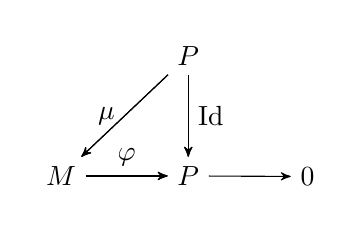
\begin{tikzpicture}% Fix later by making mu dashed
  \matrix (m) [matrix of math nodes, row sep=3em, column sep=3em]
    {  & P  &   \\
      M & P & 0 \\ };
  { [start chain];
    \chainin (m-1-2);
    { [start branch=P] \chainin (m-2-1)
        [join={node[left] {$\mu  $}}];}
    { [start branch=P'] \chainin (m-2-2)
	[join={node[right] {$\textrm{Id} $}}];}}
  { [start chain] \chainin (m-2-1);
    \chainin (m-2-2) [join={node[above] {\(\varphi \)}}];
    \chainin (m-2-3) ;}
\end{tikzpicture}
\end{center}
	\item If \(P\) is a quotient of the \(R\)-module \(M\) then \(P\) is isomorphic to a direct summand of \(P\). That is, every short exact sequence
		\begin{align*}
			0\to L \to M\to P\to 0
		\end{align*}
		splits.
	\item \(P\) is a direct summand of a free \(R\)-module.
	\end{itemize}
\end{prop}

\begin{defn}[Projective Modules]
	An \(R\)-module \(\prescript{}{R}P\) is called \textbf{projective} if any module \(M\) that projects onto \(P\) has an isomorphic copy of \(P\) as a direct summand.
\end{defn}
A projective module is merely one that satisfies any of the above equivalent conditions.

\begin{cor}
	Free modules are projective modules.\\

	A finitely generated module is projective if and only if it is the direct summand of a finitely generated free module.\\

	Every free module is a quotient of a projective module.
\end{cor}

\begin{exmp}
	
\end{exmp}

% Category theory explanation and functors

\subsection{Injective Modules}
\label{sub:injective_modules}

Of course we can also consider the reverse case-- when do \(R\)-module homomorphisms from \(L\) or \(N\) to \(D\) exist?\\

We can see that an \(R\)-module map from \(N\) to \(D\) induces a map from \(M\) to \(D\) by composition by
\begin{align*}
	\varphi' : \textrm{Hom}_R(N,D) &\to \textrm{Hom}_R(M,D)\\
	f &\mapsto f' = f \circ \varphi 
\end{align*}
which is injective, and hence if the sequence
\begin{align*}
	M\to^{\varphi }N \to 0
\end{align*} is exact, then
\begin{align*}
	0 \to \textrm{Hom}_R(N,D) \to^{\varphi '} \textrm{Hom}_R(M,D)
\end{align*} is exact.\\

The reverse does not hold in general.

\begin{exmp}
	
\end{exmp}

\begin{thm}
	Let \(D,L,M,N\) form \(R\)-modules. If
	\begin{align*}
		0 \to L \to^{\psi }M \to^{\varphi }N \to 0
	\end{align*}
	is exact, then
	\begin{align*}
		0 \to \textrm{Hom}_R(N,D) \to^{\varphi '} \textrm{Hom}_R(M,D) \to^{\psi'} \textrm{Hom}_R(L,D)
	\end{align*} is exact.\\

	A homomorphism \(f:L\to D\) lifts to a homomorphism \(F:M\to D\) if and only if \(f\) is in the image of \(\psi '\).\\

	The sequence of homomorphisms is exact for all \(R\)-modules \(D\) if and only if
	\begin{align*}
		L \to^{\psi }M \to^{\varphi }N \to 0
	\end{align*}
	is exact.
\end{thm}
Hence the sequence
\begin{align*}
	0 \to \textrm{Hom}_R(N,D) \to^{\varphi '}\textrm{Hom}_R(M,D) \to^{\psi '}\textrm{Hom}_R(L,D) \to 0
\end{align*} is not a short exact sequence in general, as \(\psi '\) may not be surjective.\\

Of course, this sequence is exact if the original exact sequence is a split exact sequence (in which case the sequence of homomorphisms is a split exact sequence for every \(R\)-module \(D\)).

\begin{hw}
	If 
	\begin{align*}
		0 \to \textrm{Hom}_R(N,D) \to^{\varphi '}\textrm{Hom}_R(M,D) \to^{\psi '}\textrm{Hom}_R(L,D) \to 0
	\end{align*}
	is exact for every \(R\)-module \(D\), then
	\begin{align*}
		0 \to L \to^{\psi }M \to^{\varphi }N \to 0
	\end{align*}
	is a split short exact sequence.\\

	This implies that if the homomorphism sequence is exact for every \(D\), then it is split exact for every \(D\).
\end{hw}

\begin{prop}
	Let \(Q\) be an \(R\)-module. Then the following are equivalent:
	\begin{itemize}
		\item Let \(L,M,N\) form \(R\)-modules. If
			\begin{align*}
				0 \to L \to^{\psi }M \to^{\varphi }N \to 0
			\end{align*}
			is a short exact sequence, then
			\begin{align*}
				0 \to \textrm{Hom}_R(N,Q) \to^{\varphi '} \textrm{Hom}_R(M,Q) \to^{\psi '} \textrm{Hom}_R(L,Q) \to 0
			\end{align*}
			is also a short exact sequence.
		\item Let \(L,M\) form \(R\)-modules. If \(0 \to L\to^{\psi }M\) is exact, then every \(R\)-module homomorphism from \(L\) to \(Q\) lifts to an \(R\)-module homomorphism of \(M\) into \(Q\). That is, the following diagram commutes:
\begin{center}
\begin{tikzpicture}% Fix later by making F dashed
  \matrix (m) [matrix of math nodes, row sep=3em, column sep=3em]
    { 0 & L  & M  \\
       & Q &  \\ };
  { [start chain];
    \chainin (m-1-1);
    \chainin (m-1-2);
    { [start branch=L] \chainin (m-2-2)
    [join={node[left] {\(f\) }}];}
    \chainin (m-1-3) [join={node[above] {\(\psi \)}}];
    { [start branch=M] \chainin (m-2-2)
	[join={node[right] {$F $}}];}}
\end{tikzpicture}
\end{center}
\item If \(Q\) is a submodule of the \(R\)-module \(M\), then \(Q\) is a direct summand of \(M\). That is, every short exact sequence
	\begin{align*}
		0 \to Q \to M \to N \to 0
	\end{align*}
	splits.
	\end{itemize}
\end{prop}

\begin{defn}[Injective Modules]
	An \(R\)-module \(\prescript{}{R}Q\) is called \textbf{injective} if for any module \(M\) that \(Q\) injects into, \(M\) has an isomorphic copy of \(Q\) as a direct summand.
\end{defn}

\begin{exmp}
		
\end{exmp}

%Category theory stuff again

Unfortunately, there is not a nice equivalent to the direct summand of a free \(R\)-module condition from projective modules. Instead:
\begin{prop}[Baer's Criterion]
	Let \(Q\) form an  \(R\)-module. \(\prescript{}{R}Q\) is injective if and only if for every left ideal \(I\triangleleft R\), any \(R\)-module homomorphism \(g:I\to Q\) can be extended to an \(R\)-module homomorphism \(G:R\to Q\).
\end{prop}
If \(R\) is a PID, then \(Q\) is injective if and only if \(rQ = Q\) for every nonzero \(r \in R\). Hence, a \(\Z\)-module is injective if and only if it is divisible. When \(R\) is a PID, quotient modules of injective \(R\)-modules are injective.
\begin{proof}
	
\end{proof}

\begin{cor}
	Every \(\Z\)-module is a submodule of an injective \(\Z\)-module.
\end{cor}
This can be useful to prove the more general statement:
\begin{thm}
	Let \(R\) be a ring and \(\prescript{}{R}M\) an \(R\)-module. Then \(M\) is contained in an injective \(R\)-module.
\end{thm}

\subsection{Flat Modules}
\label{sub:flat_modules}

Suppose \(D\) forms a right \(R\)-module. For every homomorphism \(f:X\to Y\) of left \(R\)-modules, we obtain a homomorphism
\begin{align*}
	1 \otimes f: D \otimes_R X \to D \otimes_R Y
\end{align*}
of abelian groups. If \(D \) is also an \((S,R)\)-bimodule, then \(1 \otimes f\) is a homomorphism of left \(S\)-modules.

\begin{thm}
	Let \(D\) form a right \(R\)-module, and \(L,M,N\) form left \(R\)-modules. If
	\begin{align*}
		0 \to L \to^{\psi }M \to^{\varphi }N \to 0
	\end{align*}
	is exact, then
	\begin{align*}
		D \otimes_R L ^{1 \otimes \psi }D \otimes_R M \to^{1 \otimes \varphi }D \otimes_R N \to 0
	\end{align*}
	is exact.\\

	If \(D\) is an \((S,R)\)-bimodule then the sequence of abelian groups is an exact sequence of left \(S\)-modules. Hence, if \(S = R\) is commutative, then the sequence of abelian groups is an exact sequence of \(R\)-modules. The map \(1 \otimes \varphi \) is not necessarily injective, so the sequence may not extend to a short exact sequence.\\

	The sequence of abelian groups is exact for all right \(R\)-modules \(D\) if and only if
	\begin{align*}
		L \to^{\psi }M \to^{\varphi }N \to 0
	\end{align*}
	is exact.
\end{thm}

\begin{prop}
	Let \(A\) form a right \(R\)-module. Then the following are equivalent:
	\begin{itemize}
		\item Let \(L,M,N\) form left \(R\)-modules. If
			\begin{align*}
				0 \to L \to^{\psi } M \to^{\varphi }N \to 0
			\end{align*}
			is a short exact sequence, then
			\begin{align*}
				0 \to A \otimes_R L \to^{1 \otimes \psi } A \otimes_R M \to^{1 \otimes \varphi } A \otimes_R N \to 0
			\end{align*}
			is a short exact sequence.
		\item  Let \(L,M\) be left \(R\)-modules, if
			\begin{align*}
				0 \to L \to^{\psi }M
			\end{align*} is an exact sequence of left \(R\)-modules, then
			\begin{align*}
				0 \to A \otimes_R L \to^{1 \otimes \psi } A \otimes_R M
			\end{align*} is an exact sequence of abelian groups.
	\end{itemize}
\end{prop}

\begin{defn}
	A right \(R\)-module \(\prescript{}{R}A\) is called \textbf{flat} if either of the above conditions hold.
\end{defn}

\begin{cor}
	Free modules are flat. Moreover, projective modules are flat.
\end{cor}

\begin{exmp}
	
\end{exmp}

\begin{thm}
	Let \(R,S\) be rings, left \(A\) form a right \(R\)-module, let \(B\) form an \((R,S)\)-bimodule and let \(C\) form a right \(S\)-module. Then there is an isomorphism of abelian groups:
	\begin{align*}
		\textrm{Hom}_S(A \otimes_R B, C) \cong \textrm{Hom}_R(A, \textrm{Hom}_S(B,C))
	\end{align*}
\end{thm}
If \(R=S\) is commutative this is an isomorphism of \(R\)-modules with the standard \(R\)-module structures.

\begin{cor}
	If \(R\) is commutative then the tensor product of two projective \(R\)-modules is projective.
\end{cor}

\end{document}


\chapter{Structure of Modules over Principal Ideal Domains}
\label{cha:structure_of_modules_over_principal_ideal_domains}

\section{Fundamental Structure Theorems}
\label{sec:fundamental_structure_theorems}

\documentclass{memoir}
\usepackage{notestemplate}

%\logo{~/School-Work/Auxiliary-Files/resources/png/logo.png}
%\institute{Rice University}
%\faculty{Faculty of Whatever Sciences}
%\department{Department of Mathematics}
%\title{Class Notes}
%\subtitle{Based on MATH xxx}
%\author{\textit{Author}\\Gabriel \textsc{Gress}}
%\supervisor{Linus \textsc{Torvalds}}
%\context{Well, I was bored...}
%\date{\today}

%\makeindex

\begin{document}

% \maketitle

% Notes taken on 

\begin{defn}[Rank]
	Let \(R\) be an integral domain. The \textbf{rank} of an \(R\)-module \(\prescript{}{R}M\) is the maximum number of \(R\)-linearly independent elements of \(M\).
\end{defn}

In general, an \(R\)-module of finite rank may not have a basis-- this only holds when the module is a free \(R\)-module.

\begin{exmp}
	
\end{exmp}

\begin{prop}
	Let \(R\) be an integral domain and let \(\prescript{}{R}M\) be a free \(R\)-module of rank \(n< \infty\). Then any \(n+1\) elements of \(M\) are \(R\)-linearly dependent:
	\begin{align*}
		\forall (y_1,y_2,\ldots,y_{n+1}) \in M^{n+1} \; \exists (r_1,r_2,\ldots,r_{n+1})\neq (0,0,\ldots,0) \in \R^{n+1} \text{ such that}\\
		r_1y_1 + r_2y_2 + \ldots r_{n+1}y_{n+1} = 0.
	\end{align*}
\end{prop}
In other words, the rank of a submodule of \(M\) is bounded by the rank of \(M\).

\begin{defn}[Torsion Module]
	If \(R\) is an integral domain and \(\prescript{}{R}M\) an \(R\)-module, we define the \textbf{torsion module} to be the submodule of \(M\) given by
	\begin{align*}
		\textrm{Tor}(M) = \left\{x \in M \mid rx = 0 \, r\in R \text{ nonzero} \right\} .
	\end{align*}
	If \(N \leq \textrm{Tor}(M)\) is a submodule, then we say \(N\) is a \textbf{torsion submodule of \(M\)}.\\

	If \(\textrm{Tor}(M) = 0\), then \(M\) is said to be \textbf{torsion free}.
\end{defn}
\begin{defn}[Annihilator]
	For any submodule \(N\leq M\) over a ring \(R\), the \textbf{annihilator of \(N\)} is the ideal of \(R\) defined by
	\begin{align*}
		\textrm{Ann}(N) = \left\{r \in R \mid rn = 0 \quad \forall n \in N \right\} .
	\end{align*}
\end{defn}
If \(N\) is not a torsion submodule of \(M\), then \(\textrm{Ann}(N) = 0\). If \(N,L \leq M\) as submodules with \(N\subset L\), then \(\textrm{Ann}(L) \subset \textrm{Ann}(N)\).\\

Observe that if \(R\) is a PID and \(N\subset L\subset M\) with \(\textrm{Ann}(N) = (a)\) and \(\textrm{Ann}(L) = (b)\), then \(a\mid b\). Hence, the annihilator of any element \(x \in M\) divides the annihilator of \(M\).

\begin{thm}
	Let \(R\) be a Principal Ideal Domain, let \(\prescript{}{R}M\) be a free \(R\)-module of rank \(n\), and let \(N\leq M\) be a submodule. Then \(N\) is free with rank \(m\leq n\), and there exists a basis \((y_1,y_2,\ldots,y_n) \in M^{n}\) so that
	\begin{align*}
		(a_1y_1,a_2y_2,\ldots,a_my_m)
	\end{align*} is a basis of \(N\) where \(a_1,a_2,\ldots,a_m \in R\) are nonzero. Furthermore, they satisfy the divisibility relationship:
	\begin{align*}
		a_1 \mid  a_2 \mid \ldots \mid a_m.
	\end{align*}
\end{thm}

\begin{proof}
	
\end{proof}

\begin{thm}[Fundamental Theorem of Invariant Factors]
	Let \(R\) be a PID and let \(\prescript{}{R}M\) be a finitely generated \(R\)-module.
	\begin{itemize}
		\item \(M\) is isomorphic to the direct sum of finitely many cyclic modules:
			\begin{align*}
				M \cong R^{r} \oplus R / (a_1) \oplus R / (a_2) \oplus \ldots \oplus R / (a_m)
			\end{align*}
			for some \(r \in \N\) and nonzero elements \(a_1,a_2,\ldots,a_m\) of \(R\) which are nonunital and satisfy
			\begin{align*}
				a_1 \mid a_2 \mid \ldots \mid a_m.
			\end{align*}
		\item \(M\) is torsion free if and only if \(M\) is free
		\item In the decomposition
			\begin{align*}
				M \cong R^{r} \oplus R / (a_1) \oplus R / (a_2) \oplus \ldots \oplus R / (a_m)
			\end{align*}
			the torsion module is given by
			\begin{align*}
				\textrm{Tor}(M) \cong R / (a_1) \oplus R / (a_2) \oplus \ldots \oplus R / (a_m)
			\end{align*}
			and hence \(M\) is a torsion module if and only if \(r = 0\), in which case the annihilator of \(M\) is the ideal \((a_m)\).
	\end{itemize}
\end{thm}
This decomposition is unique due to the divisibility condition.

\begin{defn}[Free Rank]
	The integer \(r\) in the decomposition of an \(R\)-module \(\prescript{}{R}M\) is called the \textbf{free rank} or \textbf{Betti number} of \(M\) and the elements \(a_1,a_2,\ldots,a_m \in R\) are the \textbf{invariant factors} of \(M\).
\end{defn}

We can apply the Chinese Remainder Theorem here to decompose the cyclic modules into cyclic modules with simple annihilators.

\begin{thm}[Fundamental Theorem of Elementary Divisors]
	Let \(R\) be a PID and let \(\prescript{}{R}M\) be a finitely generated \(R\)-module. Then
	\begin{align*}
		M \cong R^{r} \oplus R / (p_1^{\alpha _1}) \oplus R / (p_2^{\alpha 2}) \oplus \ldots \oplus R / (p_t ^{\alpha _t}
	\end{align*}
	where \(r \in \N\) and \(p_1^{\alpha_1},\ldots,p_t ^{\alpha _t}\) are positive powers of primes in \(R\).\\

	The prime powers \(p_1^{\alpha _1},\ldots,p_t ^{\alpha _t}\) are called the \textbf{elementary divisors}.
\end{thm}
The elementary divisors of a module are unique.\\

Notice that the primes are not necessarily distinct. If we group together the distinct factors we can restate the theorem in a form that is also satisfied by infinitely generated modules.

\begin{thm}[Primary Decomposition Theorem]
	LLet \(R\) be a PID and let \(\prescript{}{R}M\) be a nonzero torsion \(R\)-module with nonzero annihilator \(a\). Suppose the factorization of \(a\) into distinct prime powers in \(R\) is
	\begin{align*}
		a = u p_1^{\alpha _1}p_2^{\alpha_2}\ldots p_n^{\alpha _n}
	\end{align*}
	and let
	\begin{align*}
		N_i = \left\{x \in M \mid p_i^{\alpha _i}x = 0 \right\} .
	\end{align*}
	Then \(N_i\leq M\) is a submodule with annihilator \(p_i^{\alpha _i}\) and is the submodule of \(M\) of all elements annihilated by some power of \(p_i\). Furthermore,
	\begin{align*}
		M = N_1 \oplus N_2 \oplus \ldots \oplus N_n.
	\end{align*}
	If \(M\) is finitely generated then each \(N_i\) is the direct sum of finitely many cyclic modules whose annihilators are divisors of \(p_i^{\alpha _i}\).\\

	We call the submodule \(N_i\) the \textbf{\(p_i\)-primary component of \(M\)}.
\end{thm}
Notice that the elementary divisors of a finitely generated module \(M\) are the invariant factors of the primary components of \(\textrm{Tor}(M)\).\\

\begin{lemma}
	Let \(R\) be a PID and let \(p\) be a prime in \(R\). Let \(F\) denote the field \(R / (p)\).
	\begin{itemize}
		\item If \(M = R^{r}\), then \(M / pM \cong F^{r}\).
		\item If \(M = R / (a)\) with \(a\in R\) nonzero, then if \(p\mid a\) 
			\begin{align*}
				M / pM \cong F
			\end{align*}
			Otherwise, \(M / pM \cong 0\).
		\item If
			\begin{align*}
				M = R / (a_1) \oplus R / (a_2) \oplus \ldots \oplus R / (a_k)
			\end{align*}
			where \(p\mid a_i\), then \(M / pM \cong F^{k}\).
	\end{itemize}
\end{lemma}
This is what gives us uniqueness. Tht is, two finitely generated \(R\)-modules are isomorphic if and only i they have the same free rank and lst of invariant factors (or elementary divisors).

\begin{cor}
	Let \(R\) be a PID and let \(M\) be a finitely generated \(R\)-module. The elementary divisors of \(M\) are the prime power factors of the invariant factors of \(M\). Furthermore, the largest invariant factor of \(M\) is the product of the largest distinct prime powers among the elementary divisors of \(M\).
\end{cor}
In fact, the second largest invariant factor is the product of the largest of distinct prime powers among the remaining elementary divisors of \(M\), and so on...\\

The Fundamental Theorem of Finitely Generated Abelian Groups follows directly from this by taking \(R = \Z\).

% \printindex
\end{document}


\section{Rational Canonical Form}
\label{sec:rational_canonical_form}

\documentclass{memoir}
\usepackage{notestemplate}

%\logo{~/School-Work/Auxiliary-Files/resources/png/logo.png}
%\institute{Rice University}
%\faculty{Faculty of Whatever Sciences}
%\department{Department of Mathematics}
%\title{Class Notes}
%\subtitle{Based on MATH xxx}
%\author{\textit{Author}\\Gabriel \textsc{Gress}}
%\supervisor{Linus \textsc{Torvalds}}
%\context{Well, I was bored...}
%\date{\today}

%\makeindex

\begin{document}

% \maketitle

% Notes taken on 06/09/21

Let \(V\) be a finite dimensional vector space over \(F\) with dimension \(n\), and \(T\) a fixed linear transformation of \(V\). Recall that we can view \(V\) as an \(F[x]\)-module where \(x\) acts on \(V\) as the linear transformation \(T\).\\

Because \(V\) has finite dimension over \(F\), it must be a torsion \(F[x]\)-module. Hence \(V\) is isomorphic as an \(F[x]\)-module to the direct sum of cyclic, torsion \(F[x]\)-modules.\\

When we decompose \(V\) into the invariant factor decomposition basis, we obtain the rational canonical form for the matrix for \(T\). When we use the elementary divisor decomposition, we obtain the Jordan canonical form.

\begin{defn}[Minimal Polynomial]
 The \textbf{minimal polynomial of \(T\)} is the unique monic polynomial \(m_T(x) \in F[x]\) that generates the ideal \(\textrm{Ann}(V)\) in \(F[x]\).\\

 Let \(A\) be a matrix. The \textbf{minimal polynomial of \(T\)} is the unique monic polynomial of smallest degree \(m_A(x)\) that yields the zero matrix when evaluated at \(A\).
\end{defn}

The \textbf{rational canonical form} of the linear transformation \(T\) is the isomorphism
\begin{align*}
	V \cong F[x] / (a_1(x)) \oplus F[x] / (a_2(x)) \oplus \ldots \oplus F[x] / (a_m(x))
\end{align*}
where \(a_1(x),a_2(x),\ldots,a_m(x)\) are polynomials in \(F[x]\) of positive degree such that
 \begin{align*}
	 a_1(x) \mid a_2(x) \mid \ldots\mid a_m(x)
\end{align*}
Of course, the annihilator of \(V\) is the ideal \((a_m(x))\), and so we obtain:
\begin{prop}
	The minimal polynomial \(m_T(x)\) is the largest invariant factor of \(V\).
\end{prop}

Observe that we can get a basis for the vector space \(F[x] / (a(x))\) for a fixed
\begin{align*}
	a(x) = x^{k}+ b_{k-1}x^{k-1} + \ldots + b_1 x + b_0
\end{align*}
by defining \(\overline{x}^{k}= (x \pmod{a(x)})^{k}\). The basis is then \(\left\{ 1,\overline{x},\overline{x}^2,\ldots,\overline{x}^{k-1} \right\} \) which has an action under multiplication by \(x\) given by:
\begin{align*}
	1 \mapsto \overline{x}\\
	\overline{x} \mapsto \overline{x}^2\\
	\vdots\\
	\overline{x}^{k-2}\mapsto \overline{x}^{k-1}\\
	\overline{x}^{k-1}\mapsto \overline{x}^{k} = -b_0 - b_1\overline{x} - \ldots - b_{k-1}\overline{x}^{k-1}
\end{align*}
which follows because
\begin{align*}
	\overline{x}^{k} + b_{k-1}\overline{x}^{k-1} + \ldots + b_1\overline{x}+b_0 = 0
\end{align*}
This gives us a matrix for multiplication by \(x\):
\begin{defn}[Companion Matrix]
	Let \(a(x) = x^{k}+ b_{k-1}x^{k-1}+ \ldots + b_1x + b_0\) be a monic polynomial in \(F[x]\). The \textbf{companion matrix} of \(a(x)\) is the \(k\times k\) matrix representing the matrix for multiplication by \(x\), and is of the form
	\begin{align*}
		\begin{pmatrix} 
			0 & 0 & \ldots & \ldots & -b_0\\
			1 & 0 & \ldots & \ldots & -b_1 \\
			0 & 1 & \ldots & \ldots & -b_2\\
			\vdots & \vdots &   & \ddots & \vdots\\
			0 & 0 & \ldots & 1 & -b_{k-1}
	\end{pmatrix}
	\end{align*}
	We denote the companion matrix of \(a(x)\) by \(\mathcal{C}_{a(x)}\).
\end{defn}

Now we will apply this to each of the cyclic modules in the rational canonical form of \(V\). Let \(\mathcal{B}_i\) be the set of basis elements for each cyclic factor \(F[x] / (a_i(x))\). The linear transformation \(T\) acts on \(\mathcal{B}_i\) by the companion matrix for \(a_i(x)\), and hence the union \(\mathcal{B} = \cup_{i} \mathcal{B}_i\) and the matrix of the transformation on \(V\) is the direct sum of the companion matrices.

\begin{defn}[Rational Canonical Form]
	A matrix is said to be in \textbf{rational canonical form} if it is the direct sum of companion matrices for monic polynomials \(a_1(x),\ldots,a_m(x)\) with
	\begin{align*}
		a_1(x) \mid a_2(x) \mid \ldots \mid a_m(x).
	\end{align*}
	The matrix is then of the form
	\begin{align*}
		\begin{pmatrix} 
			\mathcal{C}_{a_1(x)} & & & \\
			& \mathcal{C}_{a_2(x)} & & \\
			& & \ddots & \\
			& & & \mathcal{C}_{a_m(x)}
		\end{pmatrix}.
	\end{align*}
	The polynomials are called the \textbf{invariant factors} of the matrix, and the matrix is said to be a \textbf{block diagonal matrix} with the blocks being the companion matrices for \(a_i(x)\).\\

	A \textbf{rational canonical form} for a linear transformation \(T\) is a matrix representing \(T\) in rational canonical form.
\end{defn}
One can check that every linear transformation \(T\) has a rational canonical form that is unique.

\begin{thm}[Rational Canonical Form for Linear Transformation]
	Let \(V\) be a finite dimensional vector space over the field \(F\) and let \(T\) be a linear transformation of \(V\). Thne there is a basis for \(V\) and the matrix of \(T\) is in rational canonical form with respect to this basis. Furthermore, the rational canonical form for \(T\) is unique.
\end{thm}
We will see that this exists for every \(T\), but Jordan canonical form may not.\\

For linear transformations \(S\) and \(T\), the following are equivalent:
\begin{itemize}
	\item \(S\) and \(T\) are similar linear transformations
	\item The \(F[x]\)-modules obtained from \(V\) via \(S,T\) are isomorphic
	\item \(S\) and \(T\) have the same rational canonical form
\end{itemize}
Of course, any matrix can be translated into a rational canonical form, as each matrix corresponds to a linear transformation. The \textbf{invariant factors} of an \(n\times n\) matrix over a field \(F\) are the invariant factors of its rational canonical form.

\begin{lemma}
	Let \(a(x) \in F[x]\) be any monic polynomial. The characteristic polynomial of the companion matrix of \(a(x)\) is \(a(x)\), and if  \(M\) is given by
	\begin{align*}
		M = 
		\begin{pmatrix}
			A_1 & 0 & \ldots & 0 \\
			0 & A_2 & \ldots & 0\\
			\vdots & \vdots & \ddots & \vdots \\
			0 & 0 & \ldots & A_k
		\end{pmatrix} 
	\end{align*}
	then the characteristic polynomial of \(M\) is the product of the characteristic polynomials of \(A_1,A_2,\ldots,A_k\).
\end{lemma}

\begin{thm}[Cayley-Hamilton Theorem]
	Let \(A\) be an \(n\times n\) matrix over the field \(F\). The minimal polynomial of \(A\) divides the characteristic polynomial of \(A\).
\end{thm}
In fact, the characteristic polynomial of \(A\) divides some power of the minimal polynomial of \(A\).

\begin{thm}
	Let \(A\) be an \(n\times n\) matrix over the field \(F\). The \(n\times n\) matrix \(xI - A\) can be put into the diagonal form
	\begin{align*}
		\begin{pmatrix} 
			1 & & & & &\\
			  & \ddots & & & &\\
			  & & 1 & & &\\
			  & & & a_1(x) & &\\
			  & & & & \ddots & \\
			  & & & & & a_m(x)
		\end{pmatrix}
	\end{align*}
	with monic nonzero elements
	\begin{align*}
		a_1(x) \mid a_2(x) \mid \ldots \mid a_m(x).
	\end{align*}
	via the operations
	\begin{itemize}
		\item interchanging two rows or columns
		\item adding a multiple of one row or column to another
		\item multiplying any column or row by a unit in \(F[x]\)
	\end{itemize}
	The elements \(a_1(x),\ldots,a_m(x)\) are the invariant factors of \(A\).
\end{thm}

\subsection{Invariant Factor Decomposition Algorithm}
\label{sub:invariant_factor_decomposition_algorithm}

%% Fill in

\subsection{Converting an \(n\times n\) Matrix to Rational Canonical Form}
\label{sub:converting_an_n_by_n_matrix_to_rational_canonical_form}


% \printindex
\end{document}



\section{Jordan Canonical Form}
\label{sec:jordan_canonical_form}

\documentclass{memoir}
\usepackage{notestemplate}

%\logo{~/School-Work/Auxiliary-Files/resources/png/logo.png}
%\institute{Rice University}
%\faculty{Faculty of Whatever Sciences}
%\department{Department of Mathematics}
%\title{Class Notes}
%\subtitle{Based on MATH xxx}
%\author{\textit{Author}\\Gabriel \textsc{Gress}}
%\supervisor{Linus \textsc{Torvalds}}
%\context{Well, I was bored...}
%\date{\today}

%\makeindex

\begin{document}

% \maketitle

% Notes taken on 


Of course, we can create a similar representation of elementary divisors, which we will refer to as the Jordan canonical form. Unlike invariant factors however, we have to make an additional assumption-- the field \(F\) contains all the eigenvalues of the linear transformation \(T\). This is equivalent to assuming all plynomials factor completely into linear factors.\\

It follows that \(V\) is a direct sum of finitely many cyclic  \(F[x]\)-modules of the form \(F[x] / (x-\lambda)^{k}\).\\

We will choose as our basis
\begin{align*}
	\left\{ (\overline{x}-\lambda )^{k-1}, (\overline{x}-\lambda )^{k-2}, \ldots, \overline{x}-\lambda , 1 \right\} 
\end{align*}
in the quotient \(F[x] / (x-\lambda)^{k}\). Then the linear transformation of multiplication by \(x\) acts as follows:
\begin{align*}
	(\overline{x}-\lambda )^{k-1} \mapsto \lambda (\overline{x}-\lambda)^{k-1} + (\overline{x}-\lambda)^{k} = \lambda (\overline{x}-\lambda)^{k-1}\\
	(\overline{x}-\lambda )^{k-2}\mapsto \lambda (\overline{x}-\lambda)^{k-2} + (\overline{x}-\lambda)^{k-1}\\
	\vdots\\
	\overline{x}-\lambda \mapsto \lambda (\overline{x}-\lambda ) + (\overline{x}-\lambda)^2\\
	1 \mapsto \overline{x}
\end{align*}
This linear map has a corresponding matrix, of course.

\begin{defn}[Jordan Blocks]
	The \textbf{\(k\times k\) elementary Jordan matrix with eigenvalue \(\lambda \)} is the \(k\times k\) matrix corresponding to the linear transformation of multiplication by \(x\) on the Jordan canonical basis:
	\begin{align*}
		\begin{pmatrix} 
			\lambda & 1 & & & \\
				& \lambda  & \ddots & &\\
			  &  & \ddots & 1 & \\
			  &  &   & \lambda & 1\\
			  & & & & \lambda 
		\end{pmatrix} 
	\end{align*}
	We refer to a matrix of this form as a \textbf{Jordan block}.
\end{defn}

We can apply this to each of the cyclic factors of \(V\) in its elementary divisor decomposition to obtain a basis for \(V\), with respect to which the matrix for \(T\) has a special form.

\begin{defn}[Jordan Canonical Form]
	A matrix is in \textbf{Jordan canonical form} if it is of the form
\begin{align*}
	\begin{pmatrix} 
	J_1 & & &\\
	    & J_2 & & \\
	    & & \ddots & \\
	    & & & J_t
	\end{pmatrix} 
\end{align*}
where \(J_i\) are Jordan blocks.
\end{defn}
The linear transformation \(T\) is in Jordan canonical form with respect to the elementary divisor basis.

\begin{thm}
	Let \(V\) be a finite dimensional vector space over \(F \) and \(T\) a linear transformation of \(V\). If \(F\) contains all the eigenvalues of \(T\), then there is a basis for \(V\) with respect to which the matrix for \(T\) is in Jordan canonical form. Furthermore, this matrix is unique up to permutation.
\end{thm}

\begin{cor}
	If a matrix \(A\) is similar to a diagonal matrix \(D\), then \(D\) is the Jordan canonical form. Hence, two diagonal matrices are similar if and only if their diagonal entries are the same up to permutation.
\end{cor}

\begin{cor}
	If \(A\) is an \(n\times n\) matrix with entries from \(F\), and \(F\) contains all the eigenvalues of \(A\), then \(A\) is similar to a diagonal matrix over \(F\) if and only if the minimal polynomial of \(A\) has no repeated roots.
\end{cor}

\begin{exmp}
	
\end{exmp}

\subsection{Changing from one canonical field to another}
\label{sub:changing_from_one_canonical_field_to_another}

\subsection{Elementary Divisor Decomposition Algorithm}
\label{sub:elementary_divisor_decomposition_algorithm}

\subsection{Converting an \(n\times n\) matrix to Jordan canonical form}
\label{sub:converting_an_n_by_n_matrix_to_Jordan_canonical_form}




% \printindex
\end{document}


\chapter{Group Representation Theory}
\label{cha:group_representation_theory}

\section{Ties to Group Representation Theory}
\label{sec:ties_to_group_representation_theory}
\documentclass{memoir}
\usepackage{notestemplate}

%\logo{~/School-Work/Auxiliary-Files/resources/png/logo.png}
%\institute{Rice University}
%\faculty{Faculty of Whatever Sciences}
%\department{Department of Mathematics}
%\title{Class Notes}
%\subtitle{Based on MATH xxx}
%\author{\textit{Author}\\Gabriel \textsc{Gress}}
%\supervisor{Linus \textsc{Torvalds}}
%\context{Well, I was bored...}
%\date{\today}

\begin{document}

% \maketitle

% Notes taken on 02/12/21


If, when taking an \(R\)-module \(M\), we may work over a field \(K\) and modify \(M = V\) to be a \(K\)-vector space by \(K\times V\to V\). This then gives us that an \(R\)-module over \(V\) is a pair \(V\) with \(R\times V\to V\).

\begin{defn}[Group Module]
	Let \(G\) be a group. We say that a \(K\)-vector space \(V\) is a \textbf{\(G\)-module} if it comes equipped with a \(G\)-action map
	\begin{align*}
		G\times V \to V \quad (g,v) \mapsto g*v :=gv
	\end{align*}
	compatible with operations of \(G\) and \(V\) :
	\begin{enumerate}[(a).]
		\item \(e_G v = v\) 
		\item \((gh)v = g(hv)\) 
		\item \(g(v+w) = gv + gw\) 
		\item \(g(\lambda v) = \lambda (gv)\)
	\end{enumerate}
	for all \(g,h \in G\), \(v \in V\), \(\lambda \in K\).
\end{defn}
If one is given a \(G\)-module \(V\), then there is a natural group homomorphism
\begin{align*}
	\rho:G\to \textrm{End}_K(V)\\
	g\mapsto \left[ \rho g : V \to V , \; v\mapsto g * v := gv \right] 
\end{align*}
The image of \(\rho\) is inside of \(GL(V)\).

\begin{defn}
	A \textbf{\(K\)-linear representation of a group \(G\)} is a \(K\)-vector space \(V\) equipped with a group homomorphism \(\rho:G \to GL(V)\).
\end{defn}

% Save recap

\begin{defn}
	Given a representation of a group \(G\), \((V:\rho)\), its \textbf{degree} is \(\textrm{dim}V\).
\end{defn}
Note that when \(\textrm{dim}_KV=n\), we get that
\begin{align*}
	GL(V) \cong GL_n(K)
\end{align*}
as groups.

% Something about V basis and maps between them?

Representations of \(G\) of degree \(n\) over a field \(K\) are congruent to group homomorphisms \(\rho:G\to GL_n(K)\).

\begin{defn}
	For any group \(G\), the \textbf{trivial representation of \(G\) over \(K\)} is \((V=K, \rho:G\to GL_1(K)=K^{\times })\) given by \(g\mapsto 1_K\) for all \(g \in G\).
\end{defn}

% Examples

\begin{defn}
	Let \(\rho:G\to GL(V)\) and \(\rho':G\to GL(V')\) be two representatives of a group \(G\). We say that \(p\) and \(p'\) are \textbf{equivalent} or isomorphic if there exists an invertible linear transformation
	\begin{align*}
		\tau:V\to V'
	\end{align*}
	so that \(\tau\) \textbf{intertwines} with action of \(G\) :
	\begin{align*}
		\tau(\rho g(v)) = \rho'g(\tau(v)) \quad \forall g \in G, v \in V
	\end{align*}
\end{defn}

\begin{rmrk}
	\(\rho:G\to GL_n(K)\) and \(\rho':G\to GL_{n'}(K)\) are equivalent if and only if \(n = n'\) and \(\exists T \in GL_n(K)\) such that \(T\rho(g)T^{-1} = \rho'(g)\) for all \(g \in G\).
\end{rmrk}
This notion will be captured more clearly later with homomorphism/isomorphisms.
\end{document}

\documentclass{memoir}
\usepackage{notestemplate}

%\logo{~/School-Work/Auxiliary-Files/resources/png/logo.png}
%\institute{Rice University}
%\faculty{Faculty of Whatever Sciences}
%\department{Department of Mathematics}
%\title{Class Notes}
%\subtitle{Based on MATH xxx}
%\author{\textit{Author}\\Gabriel \textsc{Gress}}
%\supervisor{Linus \textsc{Torvalds}}
%\context{Well, I was bored...}
%\date{\today}

\begin{document}

% \maketitle

% Notes taken on 02/22/21

\section{Subrepresentations and Irreducibility}
\label{sec:subrepresentations_and_irreducibility}

Let \(K\) be a field and \(G\) a group. Recall that if \(\textrm{dim}_KV = n\), we can identify the group \(GL(V)\) with \(GL_n(K)\), the group of invertible \(K \)-linear operators on \(V\) under composition.

\begin{defn}[Subrepresentations]
	Let \(\rho:G\to GL(V)\) be a representation of \(G\). Suppose that \(W\) is a subspace of \(V\) which is \(G\)-invariant. That is, for all \(w \in W\), \(g \in G\), it holds that  \(\rho_g(w)\in W\). Then \(W\) becomes a representation of \(G\) and we say that
	\begin{align*}
		(W,\rho w:G\to GL(W))\\
		g\mapsto \left[ \rho_g\mid W:W\to W \quad w \mapsto \rho_g(w) \right] 
	\end{align*}
	is a \textbf{subrepresentation} of \((V,\rho)\).
\end{defn}

% Examples

\begin{defn}
	The \textbf{direct sum} of two representations of \(G\), \((V',\rho_V')\) and \((V'',\rho_V'')\) is the representation of \(G\) given by:
	\begin{align*}
		(V:=V'\bigoplus V'', \rho_{V'\bigoplus V''}:G \to GL(V) )\\
		g\mapsto \left[ \rho_g:V\to V \quad v = v'+v''\mapsto \rho_g'(v') + \rho_g''(v'') \right] 
	\end{align*}
\end{defn}
If we fix a basis for both \(V'\) and \(V''\), then their union is a basis of \(V = V'\bigoplus V''\).

% Examples

\begin{defn}[Irreducible]
	A representation is called \textbf{irreducible} if it contains no proper subrepresentations-- otherwise it is called \textbf{reducible}. A representation is called \textbf{completely reducible} if it decomposes as a direct sum of irreducible subrepresentations.
\end{defn}
Irreducible representations will turn out to be the building blocks of group representation theory. This is complemented by Mascinke's Theorem, which will state that every \(\C\)-linear representation of a finite group \(G\) of finite degree is completely reducible.

% Example (Necessary)

\end{document}

\documentclass{memoir}
\usepackage{notestemplate}

%\logo{~/School-Work/Auxiliary-Files/resources/png/logo.png}
%\institute{Rice University}
%\faculty{Faculty of Whatever Sciences}
%\department{Department of Mathematics}
%\title{Class Notes}
%\subtitle{Based on MATH xxx}
%\author{\textit{Author}\\Gabriel \textsc{Gress}}
%\supervisor{Linus \textsc{Torvalds}}
%\context{Well, I was bored...}
%\date{\today}

\begin{document}

% \maketitle

% Notes taken on 02/24/21

\section{Complete Reducibility}
\label{sec:complete_reducibility}

Recall that the \textbf{characteristic} of a field \(K\) is the smallest positive integer \(p\) such that \(p 1_K = 0\). If \(p\) exists, then it is prime; else we say \(K\) has characteristic 0.

\begin{thm}
	Let \((V,\rho)\) be a representation of a finite group \(G\) of finite degree \(n\) over a field \(K\) of characteristic \(p\) with \(p \not\mid \left| G \right| \). If \(W\) is a subrepresentation of \((V,\rho)\), then there exists another subrepresentation \(W'\) of \(V\) so that
	\begin{align*}
		V \cong W \bigoplus W'
	\end{align*}
	as \(K\)-vector spaces. We refer to \(W'\) as the \textbf{complement} of the subrepresentation \(W\) of \((V,\rho)\).
\end{thm}

\begin{cor}[Maschke's Theorem]
	Let \(V\) be a representation of a finite group \(G\) of finite degree over a field of characteristic \(p\) with \(p \not\mid \left| G \right| \). Then \(V\) is completely reducible.
\end{cor}

This can be proven by induction on \(\textrm{dim}V\). Note that this fails for infinite groups.

\end{document}

\documentclass{memoir}
\usepackage{notestemplate}

%\logo{~/School-Work/Auxiliary-Files/resources/png/logo.png}
%\institute{Rice University}
%\faculty{Faculty of Whatever Sciences}
%\department{Department of Mathematics}
%\title{Class Notes}
%\subtitle{Based on MATH xxx}
%\author{\textit{Author}\\Gabriel \textsc{Gress}}
%\supervisor{Linus \textsc{Torvalds}}
%\context{Well, I was bored...}
%\date{\today}

\begin{document}

% \maketitle

% Notes taken on 02/26/21

\section{G-homomorphisms}
\label{sec:g_homomorphisms}

Let \(K\) be a field and \(G\) be a group. We are going to look at a structure of interest: we define \(K\)-linear representations of \(G\) as a \(K\)-vector space \(V\) equipped with a group homomorphism
\begin{align*}
	\rho:G\to GL(V)\\
	g\mapsto [\rho g:V\to V]
\end{align*}

\begin{defn}[\(G\)-homomorphism]
	Let \((V',\rho')\) and \((V'',\rho'')\) be representations of \(G\) over \(K\). A \textbf{\(G\)-homomorphism from \((V',\rho')\) to \(V'',\rho'')\)} is a \(K\) linear map \(\varphi:V'\to V''\) which intertwines with the action of \(G\) :
	\begin{align*}
		\varphi(\rho'g(v')) = \rho''g(\varphi(v')) \quad \forall g \in G, v' \in V'
	\end{align*}
	We denote the collection of \(G\)-homomorphisms from \((V', \rho')\) to \((V'', \rho'')\) by \( \textrm{Hom}_G(V',V'')\), and \(\textrm{End}_G(V') := \textrm{Hom}_G(V',V')\). Finally, a \textbf{\(G\)-isomorphism} is an invertible \(G\)-homomorphism.
\end{defn}

This is really just a change in basis.

\begin{prop}
	If \(\varphi \in \textrm{Hom}_G(V,W)\), then \(\varphi^{-1} \in \textrm{Hom}_G(W,V)\).
\end{prop}
\begin{prop} %Exercise 1 on HW 5
	Take \(\varphi \in \textrm{Hom}_G(V,W)\). Then
	\begin{enumerate}[(a).]
		\item \(\textrm{Ker}\varphi \) is a subrepresentation of \(V\), and
		\item \(\textrm{Im}\varphi\) is a subrepresentation of \(W\).
	\end{enumerate}
\end{prop}
For the rest of the section, we take \(K = \C\).

\begin{lemma}[Schur's Lemma]
	Let \((V,\rho)\) be an irreducible representation of \(G\). If \(\varphi \in \textrm{End}_G(V)\), then \(\varphi\) is a scalar multiple of \(\textrm{Id}V\) :
	\begin{align*}
		\exists \lambda \in \C \; s.t. \; \varphi(v) = \lambda v \quad \forall v \in V
	\end{align*}
\end{lemma}
This result has many applications.
\begin{thm}
	All nonzero complex irreducible representations of an abelian group \(G\) have degree 1.
\end{thm}
Using these tools, we now can complete a few problems.

\begin{hw}
	Given a finite abelian group \(G\), describe its irreducible representations, up to equivalence. Illustrate this for the Klein-four group \(G = C_2\times C_2\).
\end{hw}
Moreover, one can apply Schur's lemma to complete the following problem:
\begin{hw}
	Let \(V\) and \(W\) be irreducible representations of \(G\), and take \(\varphi \in \textrm{Hom}_G(V,W)\). Show that
	\begin{enumerate}[(a).]
		\item If \(V \not\cong W\), then \(\varphi\) is the zero map.
		\item If \(V \cong W\) and \(\varphi\neq 0\), then \(\varphi\) is a \(G\)-isomorphism.
	\end{enumerate}
\end{hw} % Hint: hw5 exercise 1

\end{document}

\documentclass{memoir}
\usepackage{notestemplate}

%\logo{~/School-Work/Auxiliary-Files/resources/png/logo.png}
%\institute{Rice University}
%\faculty{Faculty of Whatever Sciences}
%\department{Department of Mathematics}
%\title{Class Notes}
%\subtitle{Based on MATH xxx}
%\author{\textit{Author}\\Gabriel \textsc{Gress}}
%\supervisor{Linus \textsc{Torvalds}}
%\context{Well, I was bored...}
%\date{\today}

\begin{document}

% \maketitle

% Notes taken on ??


\section{Character Theory}
\label{sec:character_theory}

Character theory will serve as a very convenient bookkeeping tool for representations of \(G\) when \(G\) is finite. We still keep \(K = \C\).

\begin{defn}
	Let \((V,\rho)\) be a \(\C\)-representation of \(G\) of finite degree \(n\). Choose any basis of \(V\) and express \(\rho_g\) as a matrix in \(GL_n(\C)\), for all \(g \in G\). The \textbf{character of \((V,\rho)\)}, denoted \(X_V\) is the function
	\begin{align*}
		X_V:G\to \C\\
		g\mapsto \textrm{Tr}(\rho g)
	\end{align*}
	We say that \(X_V\) is \textbf{irreducible} if \((V,\rho)\) is irreducible.
\end{defn}
It turns out that characters detect irreducibility. Let \(X_V,\psi_W\) be given. We define a scalar by
\begin{align*}
	\langle X_V,\psi_W \rangle := \frac{1}{\left| G \right| }\sum_{g \in G} \overline{X_V(g)}\psi_W(g).
\end{align*}
\begin{prop}
	Let \(V\) be a representation of \(G\). Then
	\begin{align*}
		V \text{ is irreducible }\iff\langle X_V,X_V \rangle =1.
	\end{align*}
\end{prop}

Of course, we need to be sure that our construction of characters is well-defined. It turns out that they capture the properties of our representation well and are unique.

\begin{prop}
	\begin{enumerate}
		\item The definition of \(X_V\) is independent of choice of basis of \(V\)
		\item If \(V \cong W\), then \(X_V = X_W\) 
		\item If \(g,h \in G\) are conjugate, then \(X_V(g) = X_V(h)\)
	\end{enumerate}
\end{prop}

\begin{defn}
	The \textbf{character table} of \(G\) is defined as
	\begin{align*}
		\begin{bmatrix} X_{V_1}(g_1) & X_{V_1}(g_2) & \ldots & X_{V_1}(g_k)\\
		\vdots & & & \vdots \\
	X_{V_\ell}(g_1) & X_{V_\ell}(g_2) & \ldots & X_{V_\ell}(g_k)\end{bmatrix} 
	\end{align*}
\end{defn}
The number of irreducible characters of \(G\) is the same as the number of conjugacy classes of elements of \(G\). Furthermore, the character table is a square matrix with entries in \(\C\) when the rows are indexed by irreducible representations of \(G\) and the columns are indexed by conjugacy classes representations of elements of \(G\).\\

In this case, \((X_{V_i}(g_j))\) is an invertible matrix.

% Examples

\begin{prop}
	Let \((V,\rho )\) be a representation of \(G\), and take \(g \in G\). Then
	\begin{enumerate}
		\item \(X_V(e) = \textrm{dim}(V)\) 
		\item \(X_V(g)\) is a sum of roots of unity
		\item \(X_{V\oplus W}(g) = X_{V}(g) + X_{W}(g)\)
		\item \(X_V(g^{-1}) = \overline{X_V(g)}\) 
		\item \(\overline{X_V}\) is a character of \(G\)
	\end{enumerate}
\end{prop}

Let \(X_1,\ldots,X_r\) be irreducible characters of a finite group \(G\). Define
\begin{align*}
	\langle X_i, X_j \rangle := \frac{1}{\left| G \right| } \sum_{g \in G} \overline{X_i(g)}X_j(g)
\end{align*}

\begin{thm}
	\begin{enumerate}
		\item \(\langle X_i, X_j \rangle = \delta _{ij}\) 
		\item 
			\begin{align*}
				\sum_{i=1}^{r} \overline{X_i(x)}X_i(y) = \begin{cases}
					\left| C_G(x) \right| & x,y \text{ conjugate in }G\\
					0 & \text{otherwise}
				\end{cases}
			\end{align*}
	\end{enumerate}
\end{thm}
			Here, \(C_G(x)\) is the centralizer of \(x \in G\), that is, \(C_G(x) = \textrm{Stab}_x(G) = \left\{g \in G \mid g x g^{-1} = x \right\} \).

% Example

\begin{thm}
	If \(V,W\) are irreducible representations of \(G\), then
	\begin{align*}
		\langle X_V,X_V \rangle = 1\\
		\langle X_V,X_W \rangle = 0 \text{ when }V\not\cong W
	\end{align*}
\end{thm}
This shows us that characters completely determine representations, and forthermore characters completely determine irreducibility.
\end{document}




% \printindex
\end{document}
